\section{Background modeling}
\label{sec:BkgModeling}

\subsection{Blind strategy}
\label{subsec:BlindStrategy}
In the following sections, the modelling of kinematic distributions, particularly those used for BDT training, of the $t\bar{t}+\text{jets}$ background is checked by comparing the data and MC. In order to avoid observing signals or any other biases before fixing the analysis procedure, the following blinding strategy is applied. The signal-to-noise ratio ($S/B$) is calculated in each bin of each distribution for all mass hypotheses (more details in Appendix \ref{app:SignalBackgroundComparison}). The signal cross section (${\sigma}_{\text{signal}}$) on each mass hypothesis is set to 0.046 pb, which is the upper limit at 1 TeV $H^{+}$ mass point obtained from the resolved $H^{+}{\rightarrow}tb$ search \cite{HDBS-2021-02}. Therefore, it can be considered the most conservative assumption. The data in bins with $S/B>0.05$ in at least one mass hypothesis are blinded when the data is compared with MC.

\subsection{Data/MC comparison for BDT input variables}
\label{subsec:Data/MCBDTInputBeforeReweight}
Figures \ref{fig:DATAOVERMC_BDTInputs_Prefit} show the distributions of input variables for BDT training in the SR region. Data are blinded according to the blind strategy in Section \ref{subsec:BlindStrategy}. No significant difference between the data and MC is found in each variable.

\begin{figure}[H]
    \subfloat[HT\_jets] {
        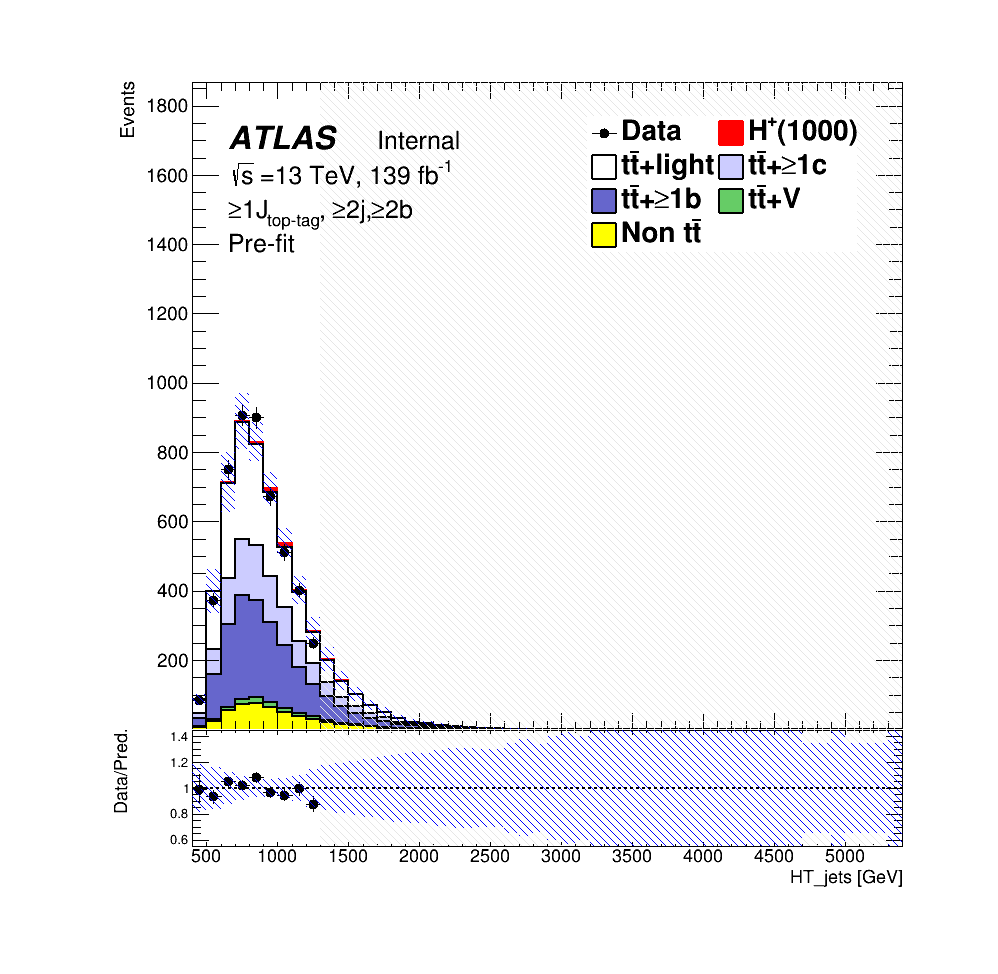
\includegraphics[width=0.50\textwidth]{images/BkgModeling/DATAOVERMC_Hp1000_Contained80_DL1r_70_HTjets_beforeRW_geq1tgeq2jgeq2b_prefit.png}
        \label{fig:DATAOVERMC_HT_jets}
    }
    \subfloat[LeadingJet\_pt] {
        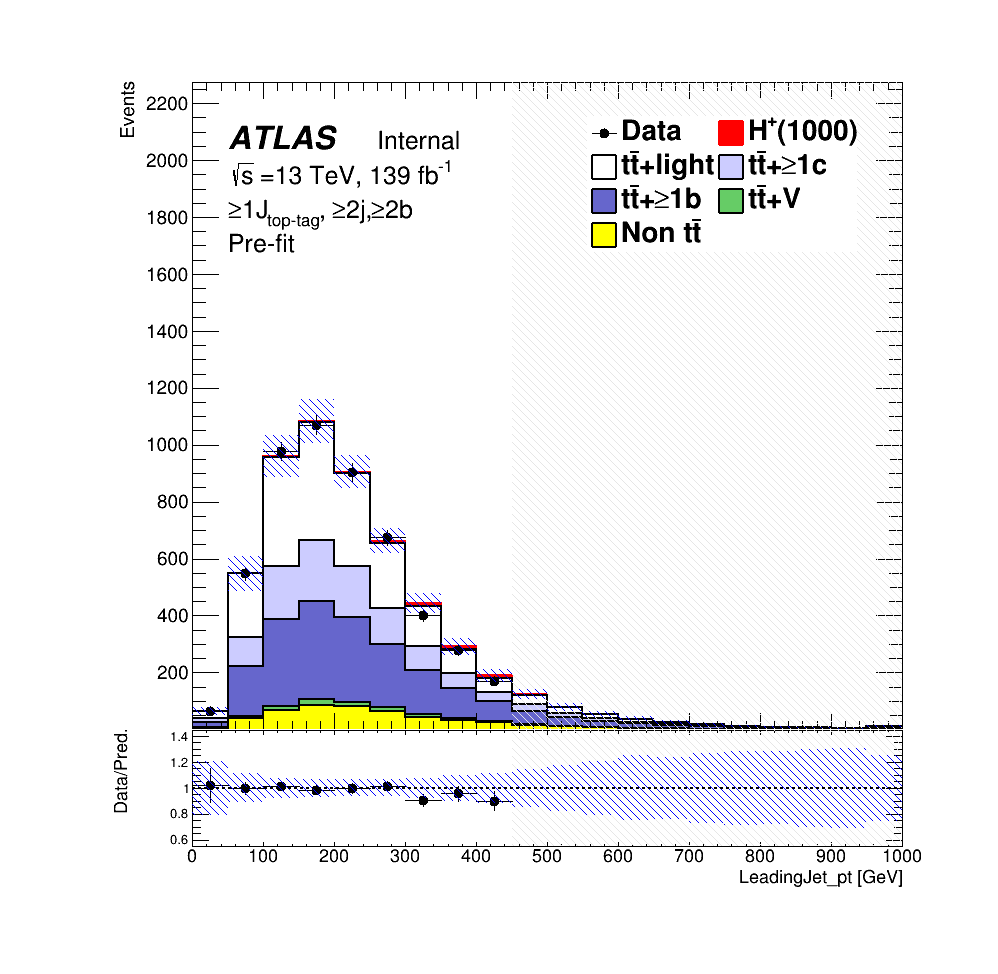
\includegraphics[width=0.50\textwidth]{images/BkgModeling/DATAOVERMC_Hp1000_Contained80_DL1r_70_LeadingJet_pt_beforeRW_geq1tgeq2jgeq2b_prefit.png}
        \label{fig:DATAOVERMC_LeadingJet_pt}
    }
\end{figure}
\begin{figure}[H]
    %\addtocounter{figure}{-1}
    \subfloat[Centrality\_all] {
        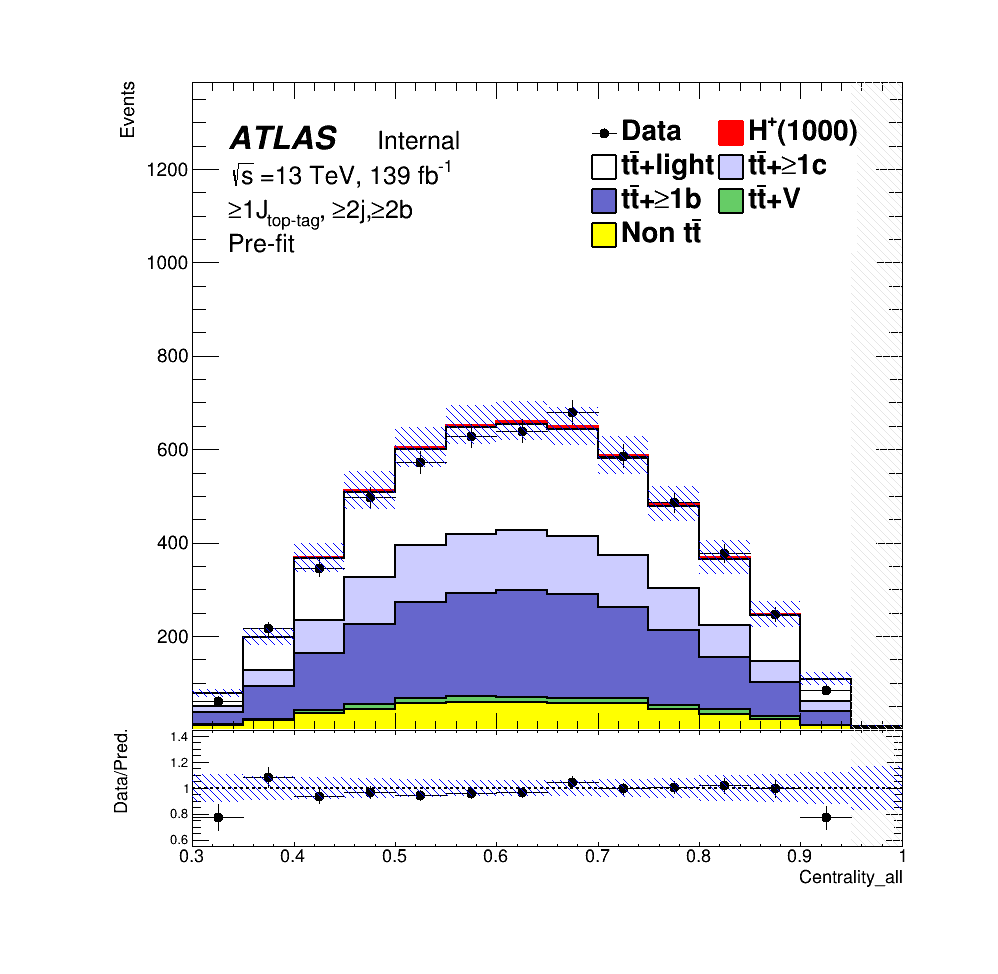
\includegraphics[width=0.50\textwidth]{images/BkgModeling/DATAOVERMC_Hp1000_Contained80_DL1r_70_Centrality_all_beforeRW_geq1tgeq2jgeq2b_prefit.png}
        \label{fig:DATAOVERMC_Centrality_all}
    }
    \subfloat[H1\_all] {
        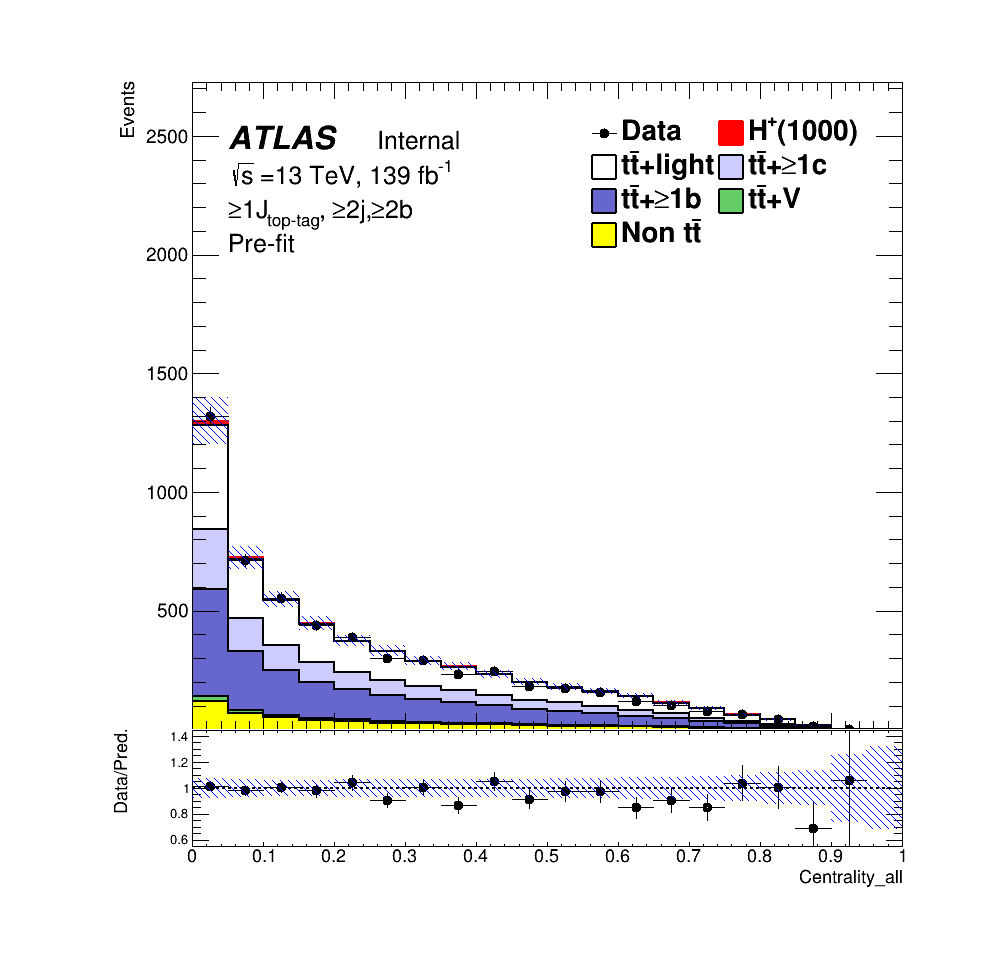
\includegraphics[width=0.50\textwidth]{images/BkgModeling/DATAOVERMC_Hp1000_Contained80_DL1r_70_H1_all_beforeRW_geq1tgeq2jgeq2b_prefit.png}
        \label{fig:DATAOVERMC_H1_all}
    }
\end{figure}
\begin{figure}[H]
    %\addtocounter{figure}{-1}
    \subfloat[Mbb\_MaxPt] {
        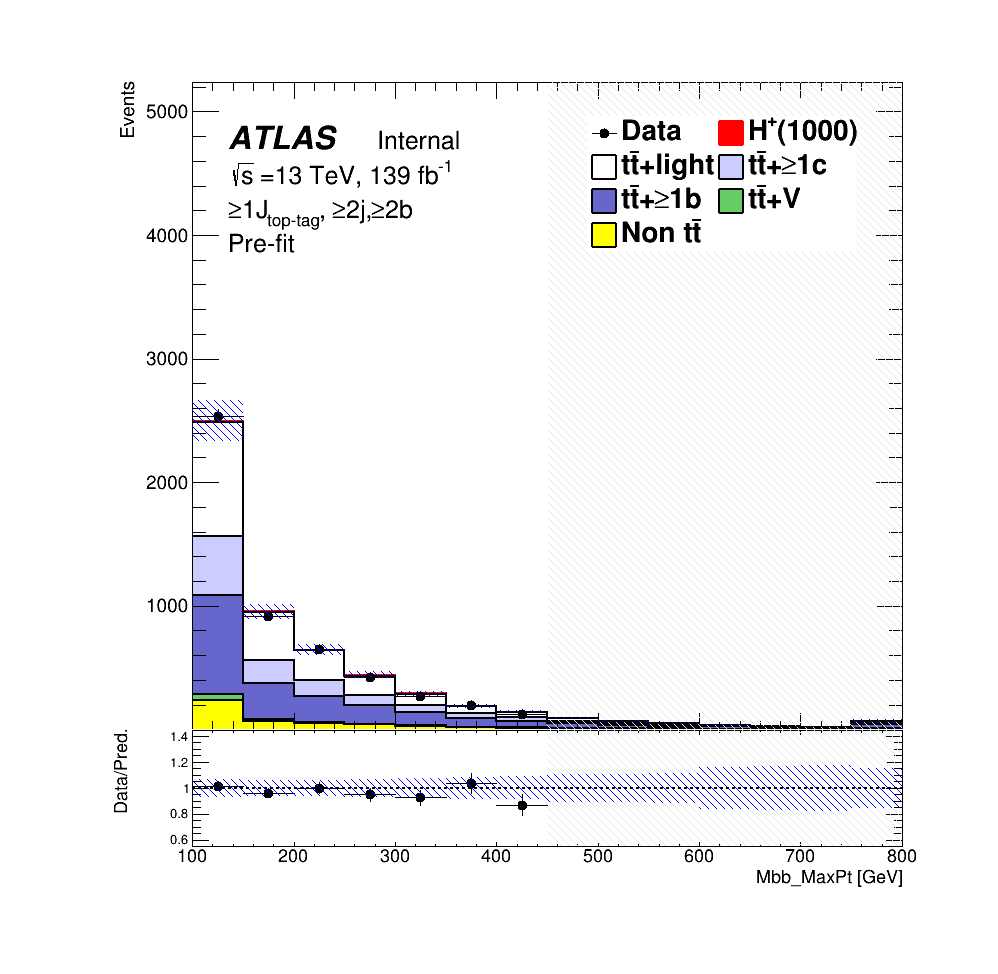
\includegraphics[width=0.50\textwidth]{images/BkgModeling/DATAOVERMC_Hp1000_Contained80_DL1r_70_Mbb_MaxPt_beforeRW_geq1tgeq2jgeq2b_prefit.png}
        \label{fig:DATAOVERMC_Mbb_MaxPt}
    }
    \subfloat[Mjjj\_MaxPt] {
        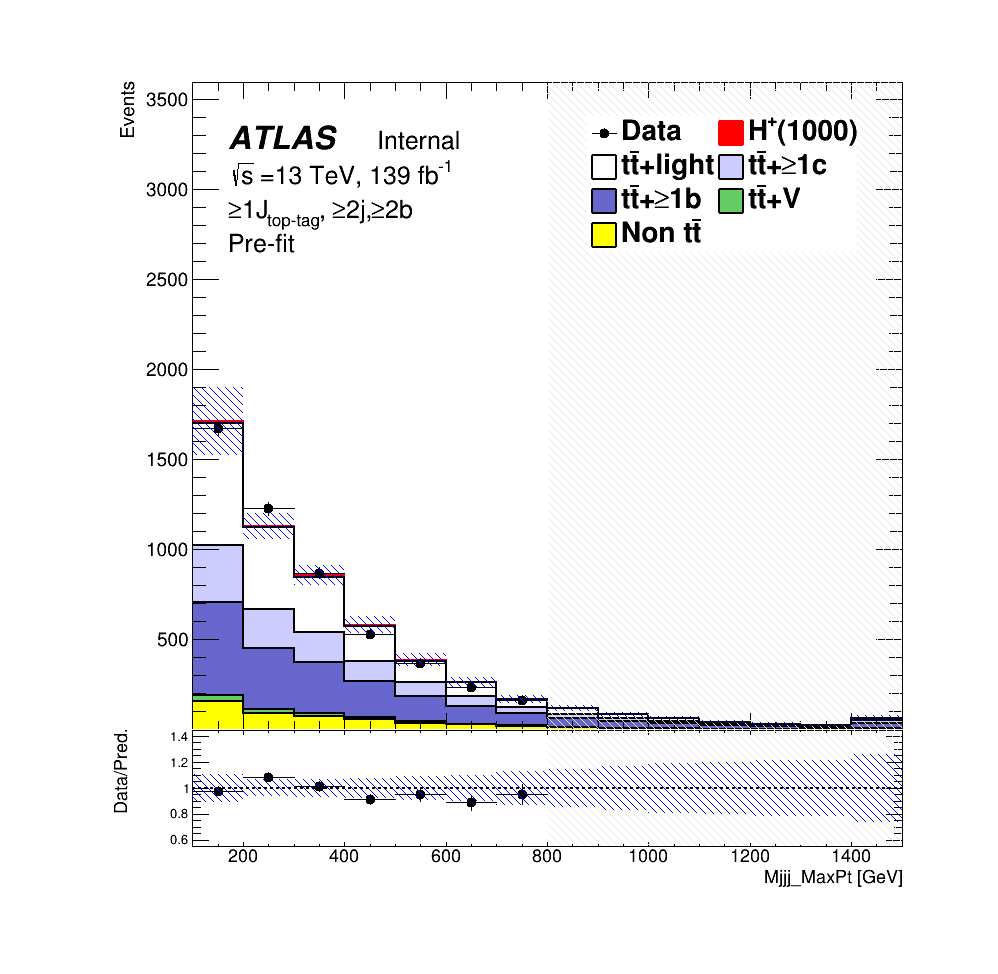
\includegraphics[width=0.50\textwidth]{images/BkgModeling/DATAOVERMC_Hp1000_Contained80_DL1r_70_Mjjj_MaxPt_beforeRW_geq1tgeq2jgeq2b_prefit.png}
        \label{fig:DATAOVERMC_Mjjj_MaxPt}
    }
\end{figure}
\begin{figure}[H]
    %\addtocounter{figure}{-1}
    \subfloat[Muu\_MindR] {
        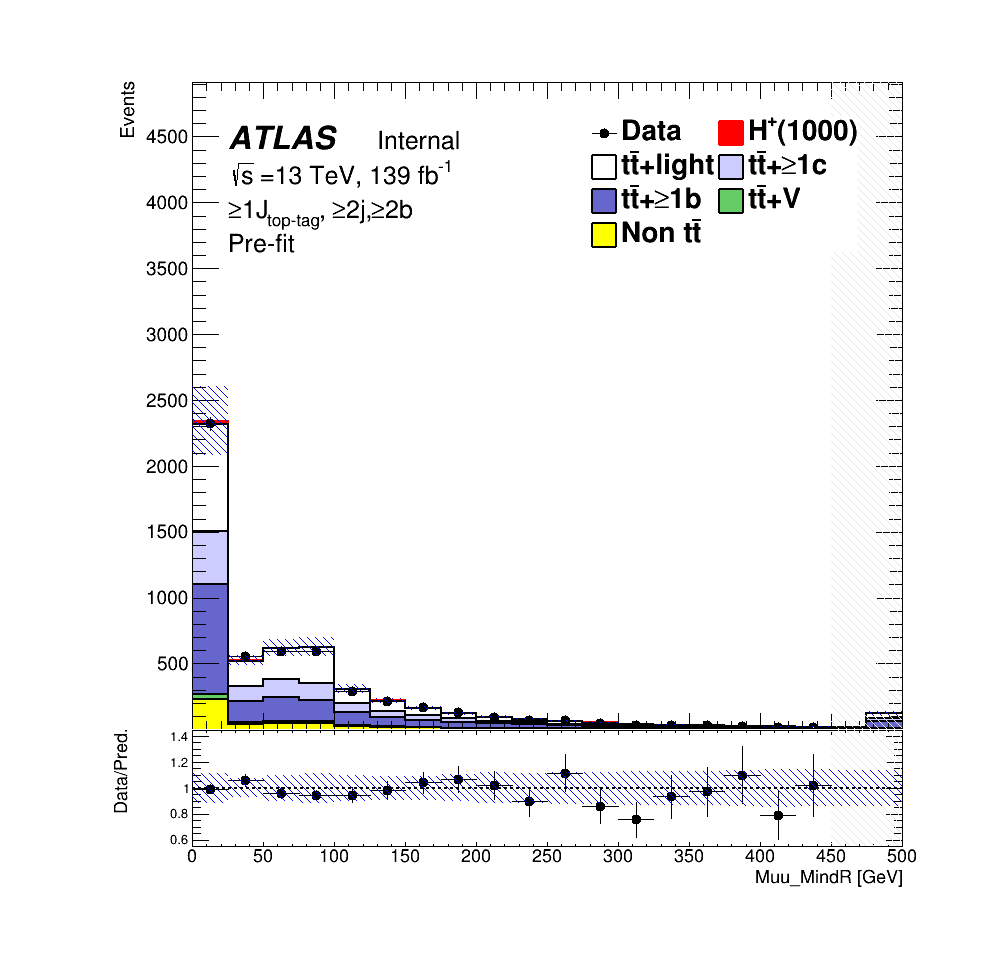
\includegraphics[width=0.50\textwidth]{images/BkgModeling/DATAOVERMC_Hp1000_Contained80_DL1r_70_Muu_MindR_beforeRW_geq1tgeq2jgeq2b_prefit.png}
        \label{fig:DATAOVERMC_Muu_MindR}
    }
    \subfloat[dRbb\_avg] {
        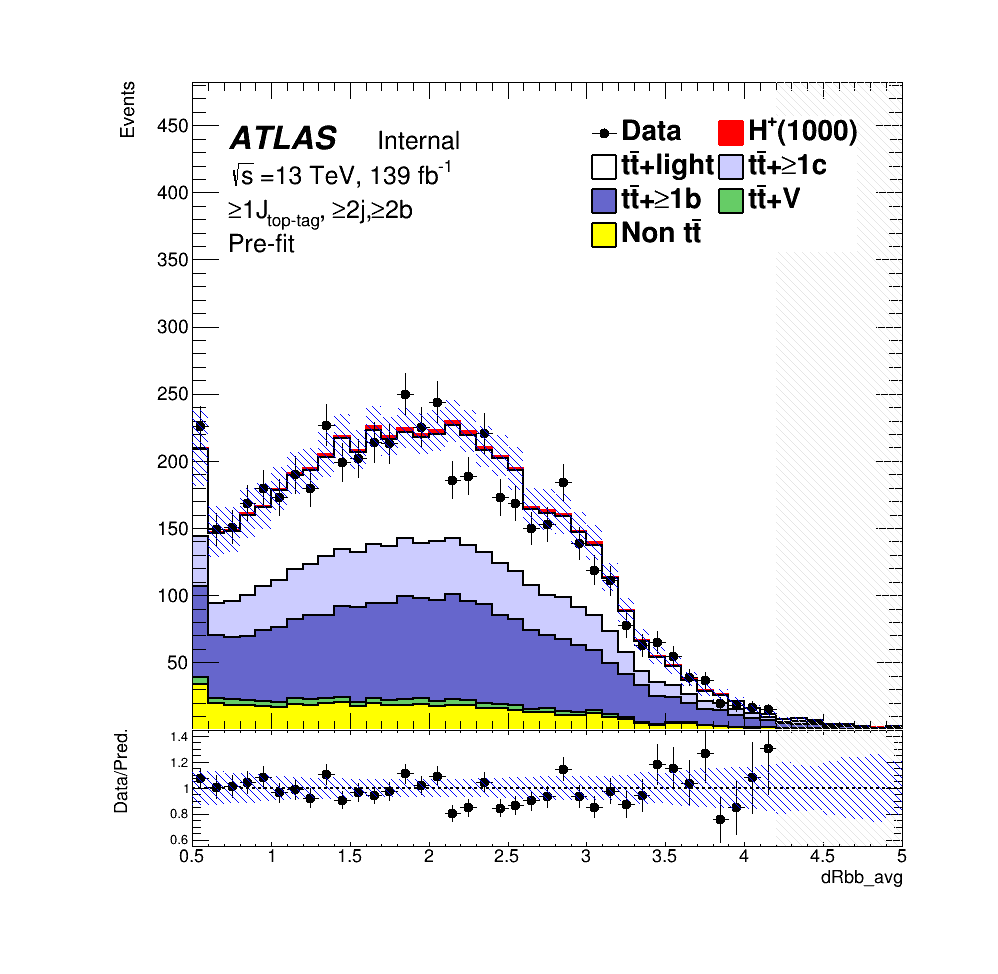
\includegraphics[width=0.50\textwidth]{images/BkgModeling/DATAOVERMC_Hp1000_Contained80_DL1r_70_dRbb_avg_beforeRW_geq1tgeq2jgeq2b_prefit.png}
        \label{fig:DATAOVERMC_dRbb_avg}
    }
\end{figure}
\begin{figure}[H]
    %\addtocounter{figure}{-1}
    \subfloat[dRlepbb\_MindR] {
        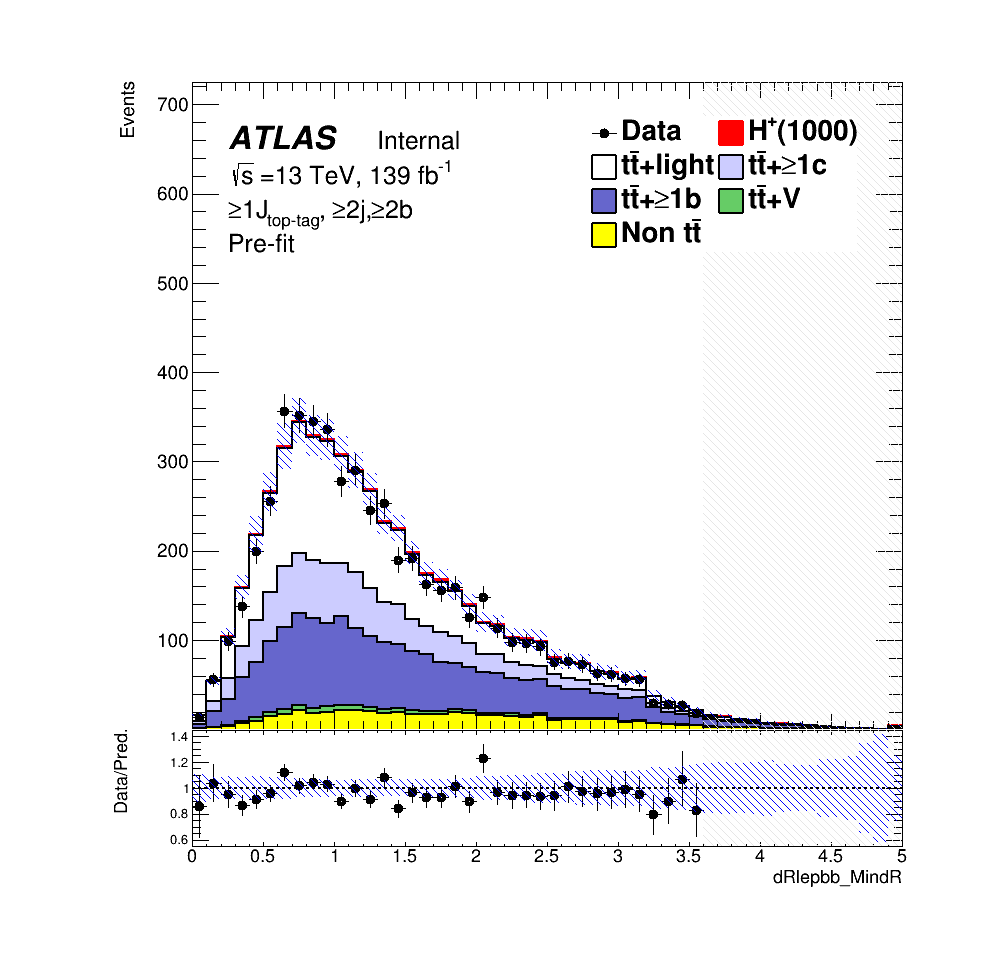
\includegraphics[width=0.50\textwidth]{images/BkgModeling/DATAOVERMC_Hp1000_Contained80_DL1r_70_dRlepbb_MindR_beforeRW_geq1tgeq2jgeq2b_prefit.png}
        \label{fig:DATAOVERMC_dRlepbb_MindR}
    }
    \subfloat[LeadingTop\_m] {
        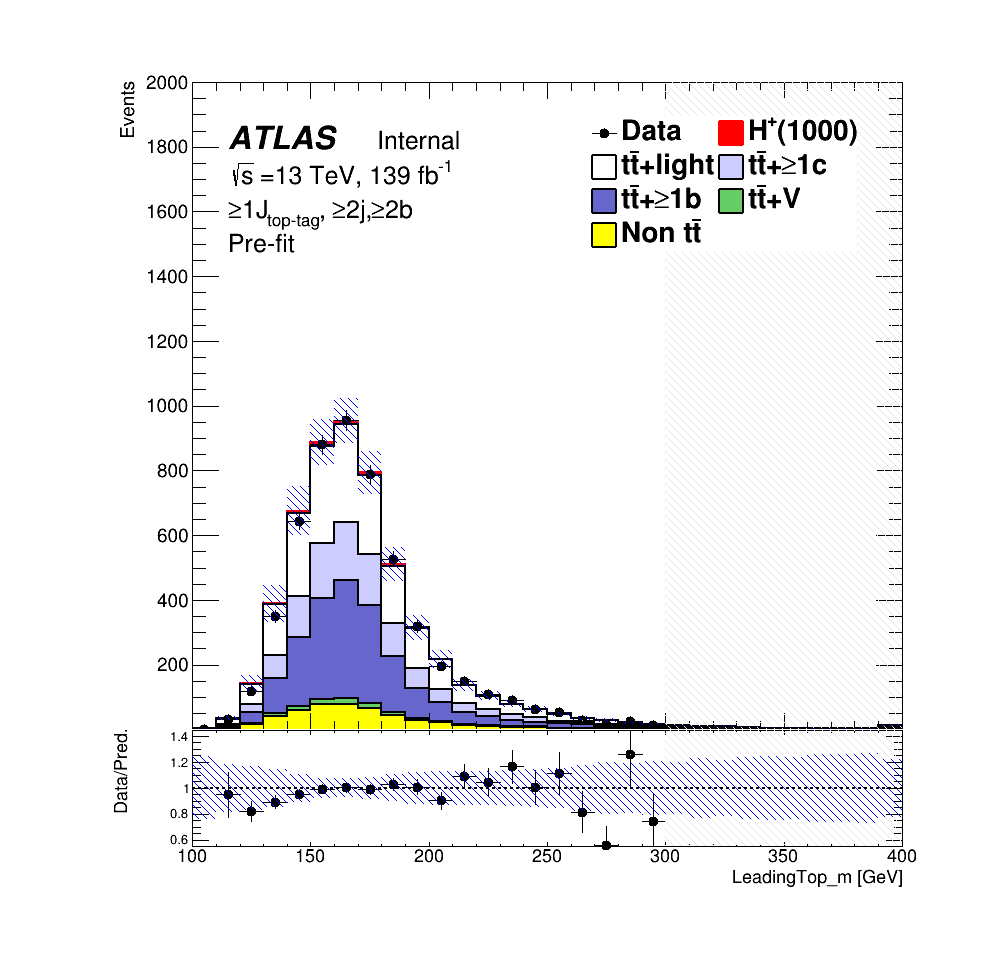
\includegraphics[width=0.50\textwidth]{images/BkgModeling/DATAOVERMC_Hp1000_Contained80_DL1r_70_LeadingTop_mass_beforeRW_geq1tgeq2jgeq2b_prefit.png}
        \label{fig:DATAOVERMC_LeadingTop_mass}
    }
\end{figure}
\begin{figure}[H]
    %\addtocounter{figure}{-1}
    \subfloat[LeadingTop\_pt] {
        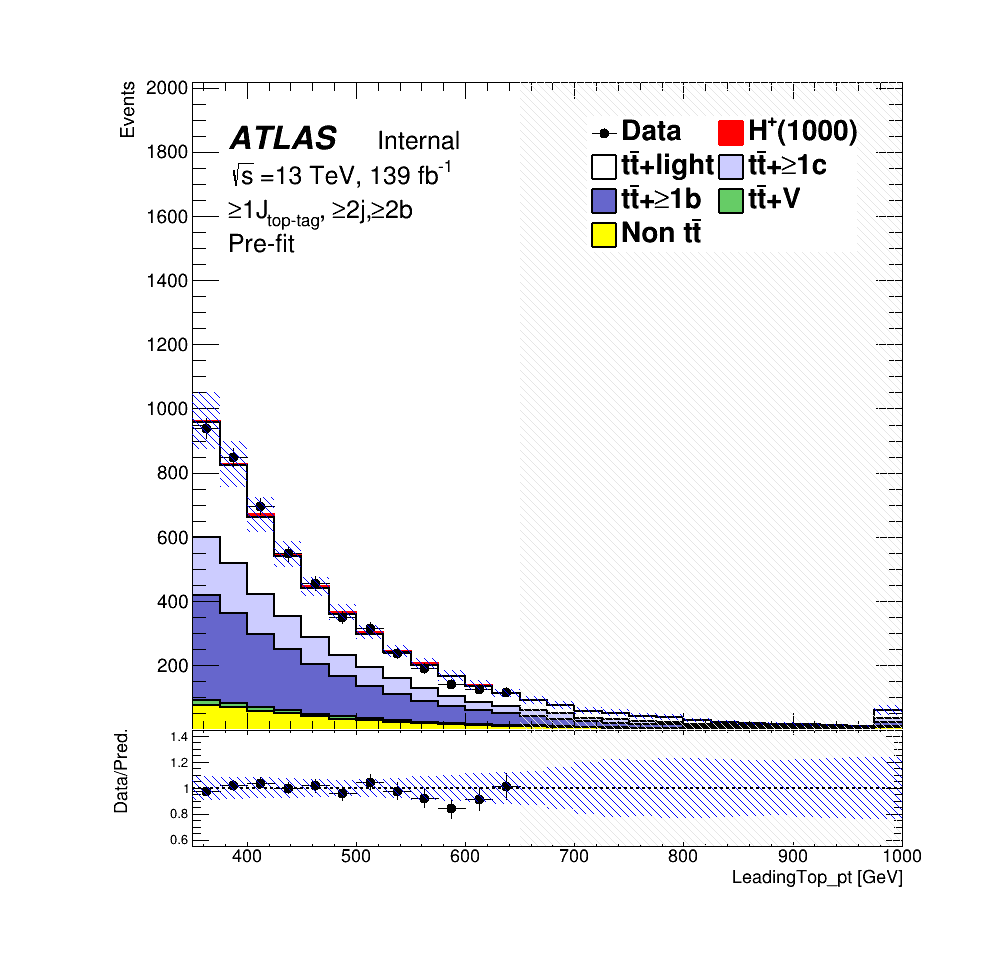
\includegraphics[width=0.50\textwidth]{images/BkgModeling/DATAOVERMC_Hp1000_Contained80_DL1r_70_LeadingTop_pt_beforeRW_geq1tgeq2jgeq2b_prefit.png}
        \label{fig:DATAOVERMC_LeadingTop_pt}
    }
    \subfloat[M\_tb] {
        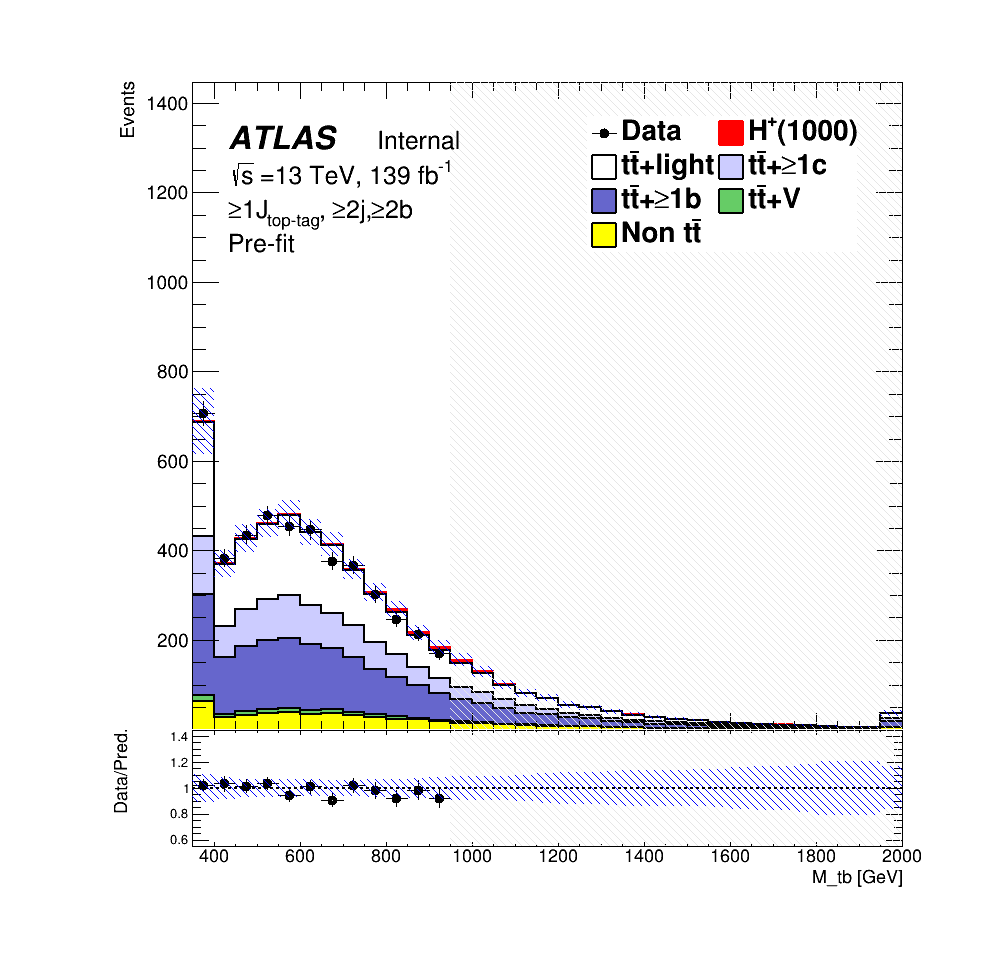
\includegraphics[width=0.50\textwidth]{images/BkgModeling/DATAOVERMC_Hp1000_Contained80_DL1r_70_tb_mass_beforeRW_geq1tgeq2jgeq2b_prefit.png}
        \label{fig:DATAOVERMC_tb_mass}
    }
\end{figure}
\begin{figure}[H]
    %\addtocounter{figure}{-1}
    \subfloat[Pt\_tb] {
        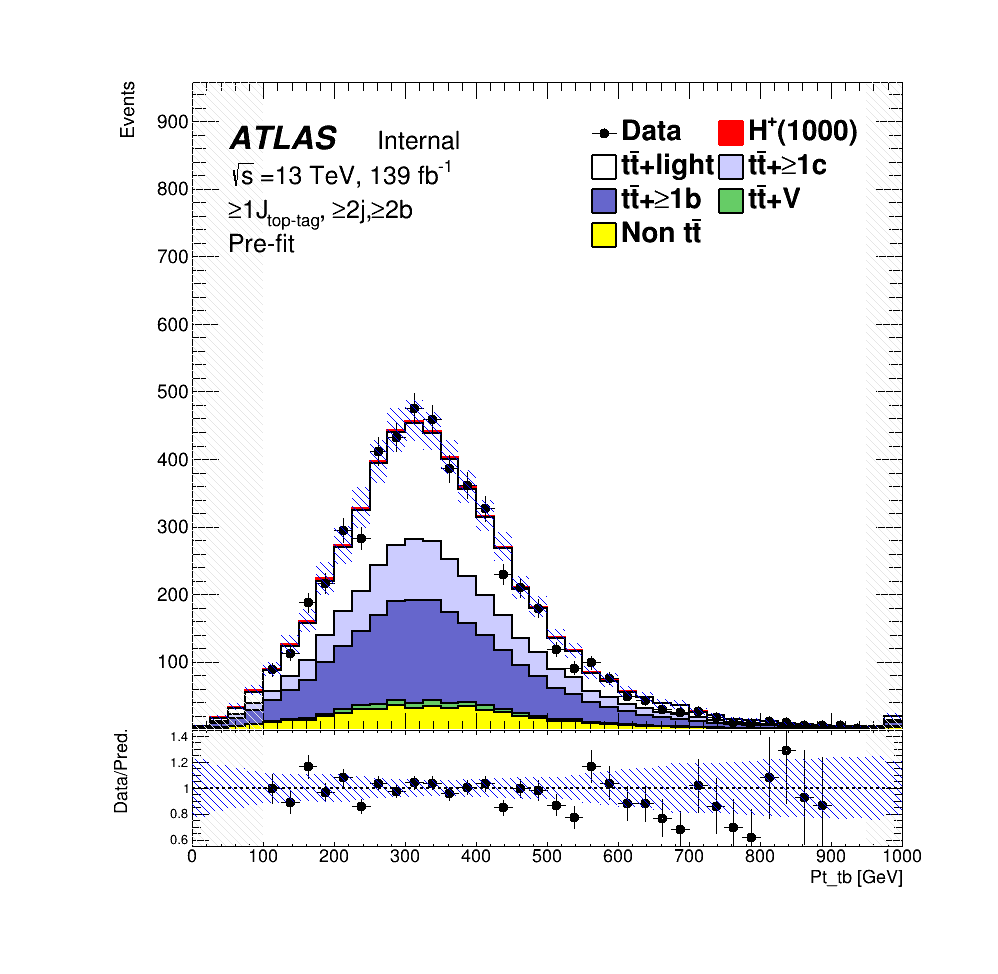
\includegraphics[width=0.50\textwidth]{images/BkgModeling/DATAOVERMC_Hp1000_Contained80_DL1r_70_tb_pt_beforeRW_geq1tgeq2jgeq2b_prefit.png}
        \label{fig:DATAOVERMC_tb_pt}
    }
    \subfloat[PtAsymm\_tb] {
        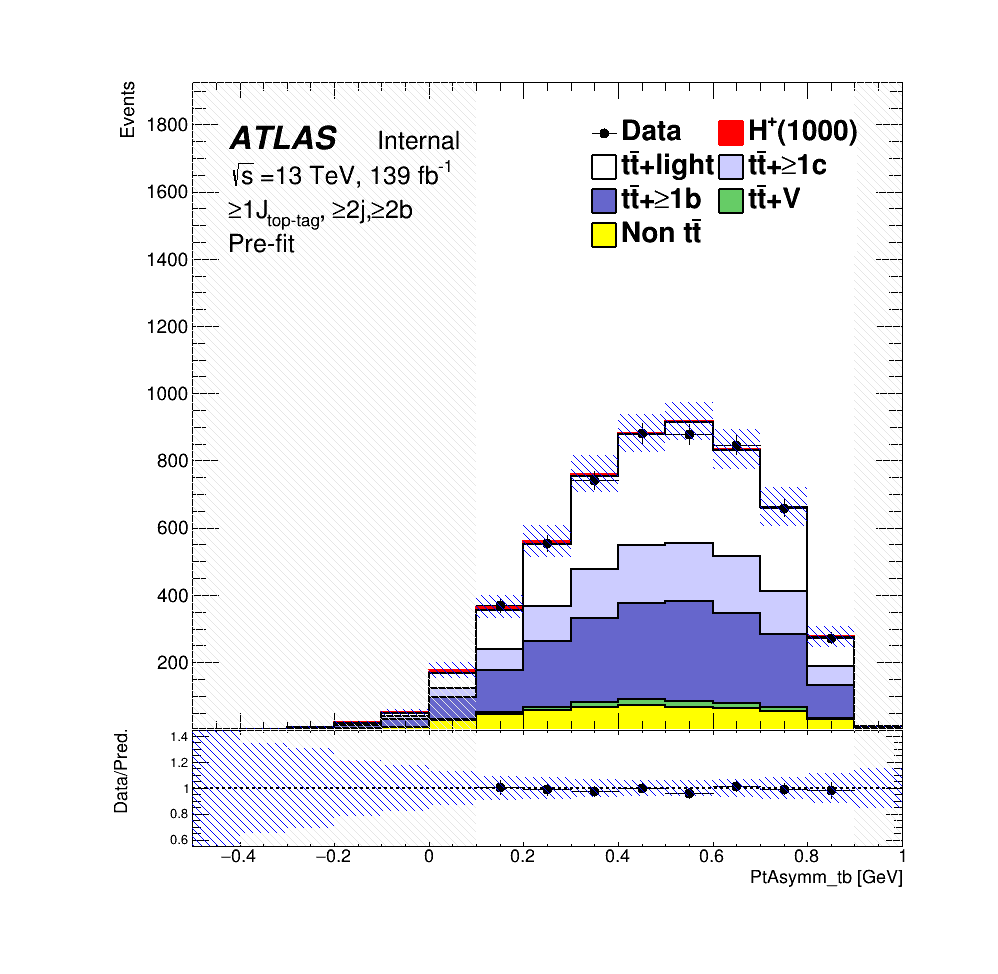
\includegraphics[width=0.50\textwidth]{images/BkgModeling/DATAOVERMC_Hp1000_Contained80_DL1r_70_tb_ptAsymm_beforeRW_geq1tgeq2jgeq2b_prefit.png}
        \label{fig:DATAOVERMC_tb_ptAsymm}
    }
  \caption{Comparison of the kinematic variables included in the BDT in the SR for the data and MC.}
  \label{fig:DATAOVERMC_BDTInputs_Prefit}
\end{figure}


\subsection{Data/MC comparison for BDT outputs}
\label{subsec:DataAndMCComparisonOfBDT}
Figures \ref{fig:DataMCComparison_BDT_Hp1000_SR_beforeRW} to \ref{fig:DataMCComparison_BDT_Hp3000_SR_beforeRW} show the distributions of BDT output in the SR. The binning of each BDT output is optimized for the search sensitivity by \textit{TransfoD} algorithm \cite{Binning-TTHFilter}. Such binning results in extremely narrow bins towards high BDT scored, and makes the plot hard to see as shown in Figure \ref{fig:SOVERB_bdt_beforeRW_geq1tgeq2jgeq2b} in Appendix \ref{subapp:SOVERB_BDTOutput} when plotted in a usual manner. We rather show the distribution with an equal interval for each bin. The distributions are input into the profile likelihood fit on each $H^{+}$ mass hypothesis as shown in Section \ref{sec:ProfileLikelohoodFit}. It is observed that the data/MC ratio tends to be lower for the high BDT score regions, which may bias the search for the signal in the highest BDT bins. The reweighting to correct for the slope is discussed in Section \ref{subsec:ReweightingTechnique}. 

\begin{figure}[H]
    \subfloat[] {
        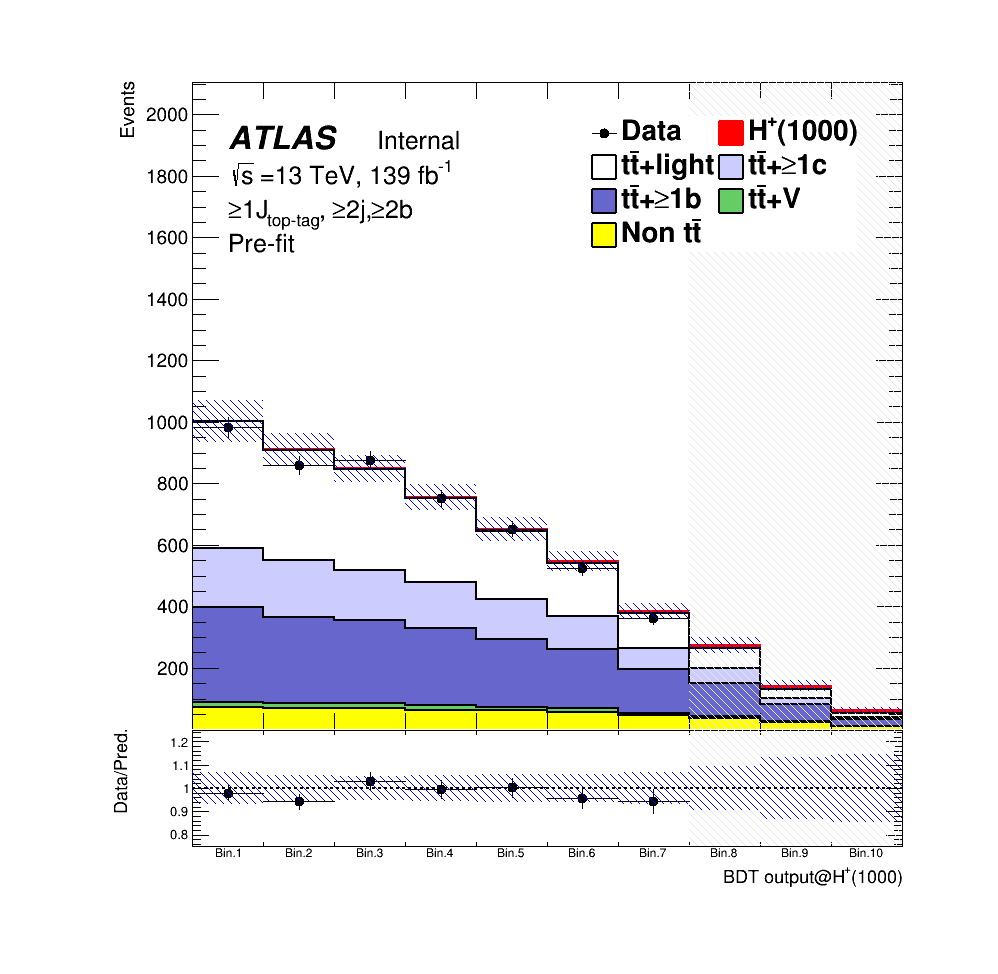
\includegraphics[width=0.50\textwidth]{images/BkgModeling/DATAOVERMC_Hp1000_Contained80_DL1r_70_bdt_Hp1000_beforeRW_geq1tgeq2jgeq2b_prefit.png}
        \label{fig:DataMCComparison_BDT_Hp1000_SR_beforeRW}
    }
    \subfloat[] {
        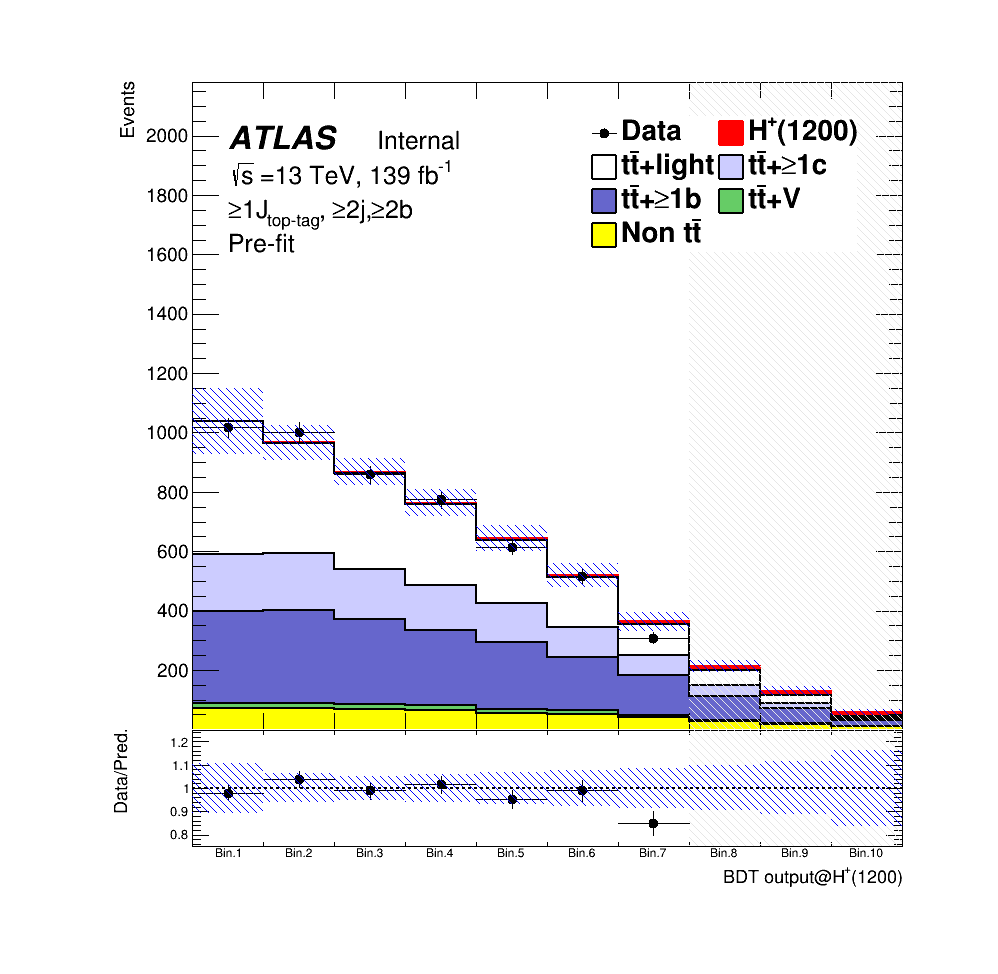
\includegraphics[width=0.50\textwidth]{images/BkgModeling/DATAOVERMC_Hp1200_Contained80_DL1r_70_bdt_Hp1200_beforeRW_geq1tgeq2jgeq2b_prefit.png}
        \label{fig:DataMCComparison_BDT_Hp1200_SR_beforeRW}
    }\par
    \subfloat[] {
        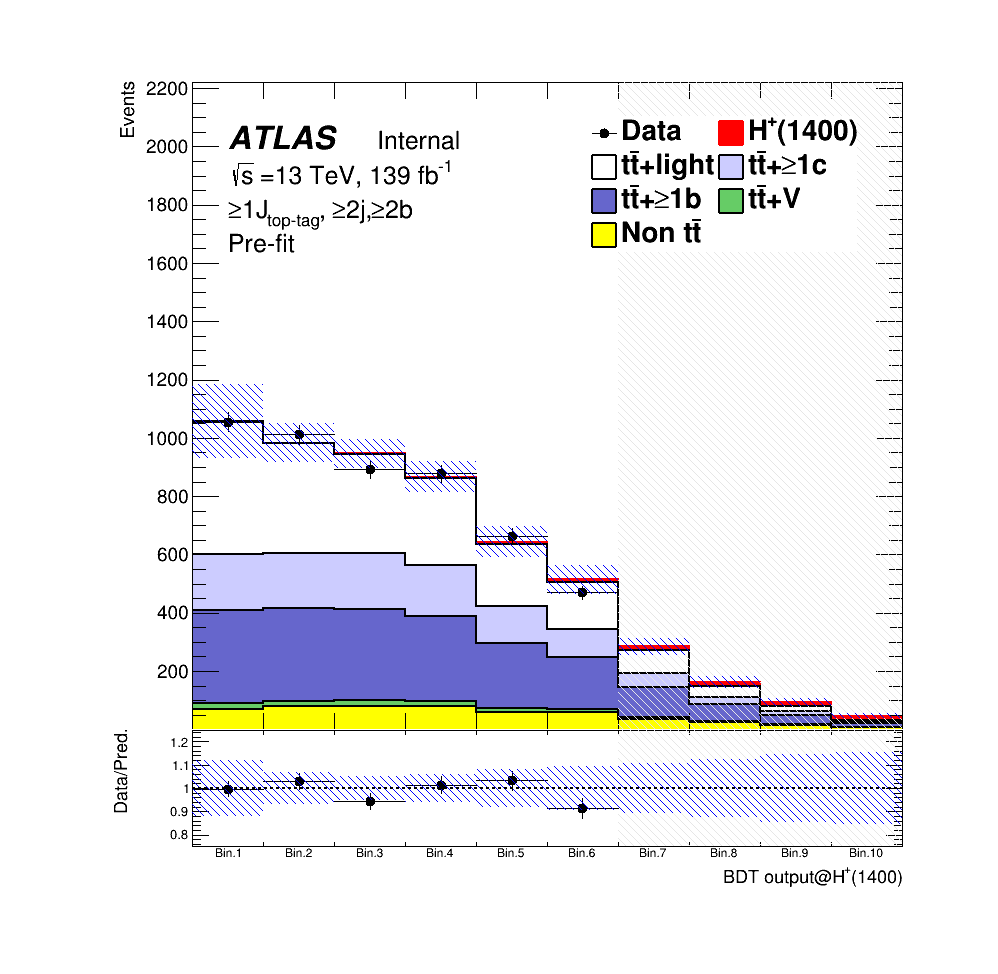
\includegraphics[width=0.50\textwidth]{images/BkgModeling/DATAOVERMC_Hp1400_Contained80_DL1r_70_bdt_Hp1400_beforeRW_geq1tgeq2jgeq2b_prefit.png}
        \label{fig:DataMCComparison_BDT_Hp1400_SR_beforeRW}
    }
    \subfloat[] {
        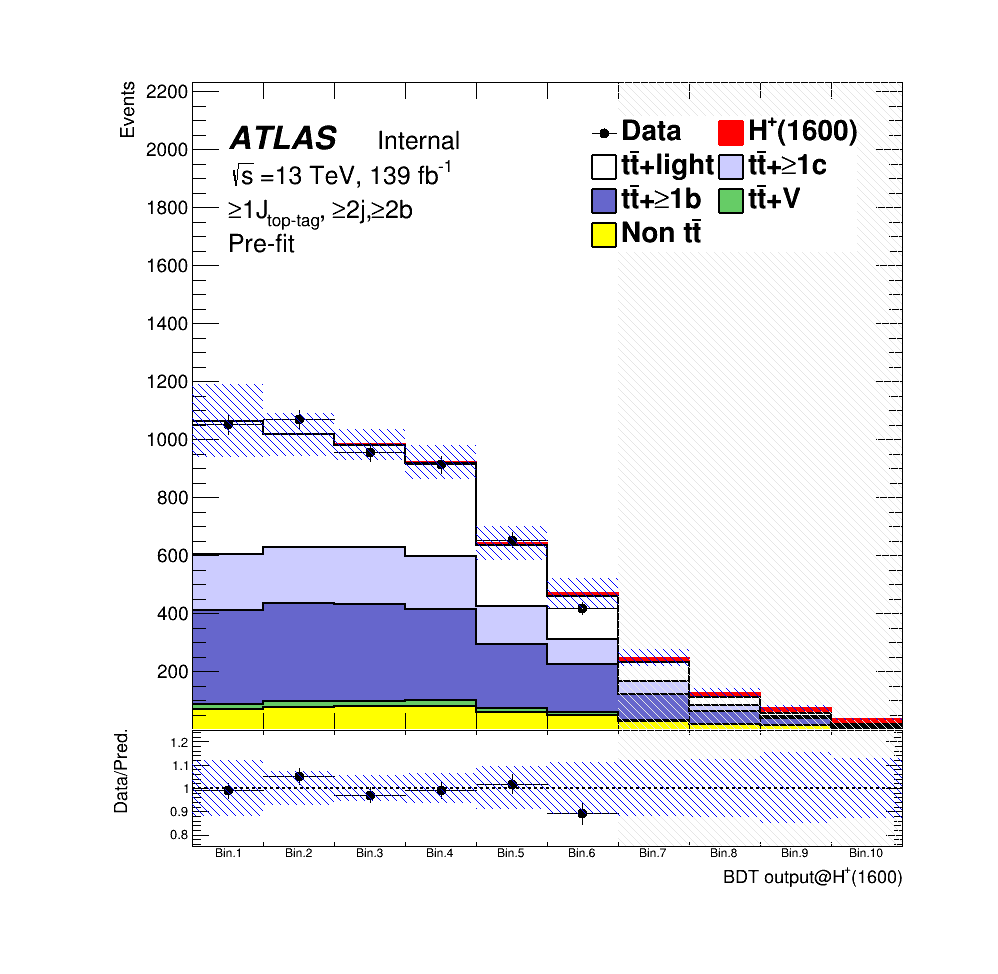
\includegraphics[width=0.50\textwidth]{images/BkgModeling/DATAOVERMC_Hp1600_Contained80_DL1r_70_bdt_Hp1600_beforeRW_geq1tgeq2jgeq2b_prefit.png}
        \label{fig:DataMCComparison_BDT_Hp1600_SR_beforeRW}
    }
\end{figure}
\begin{figure}[H]
    %\addtocounter{figure}{-1}
    \subfloat[] {
        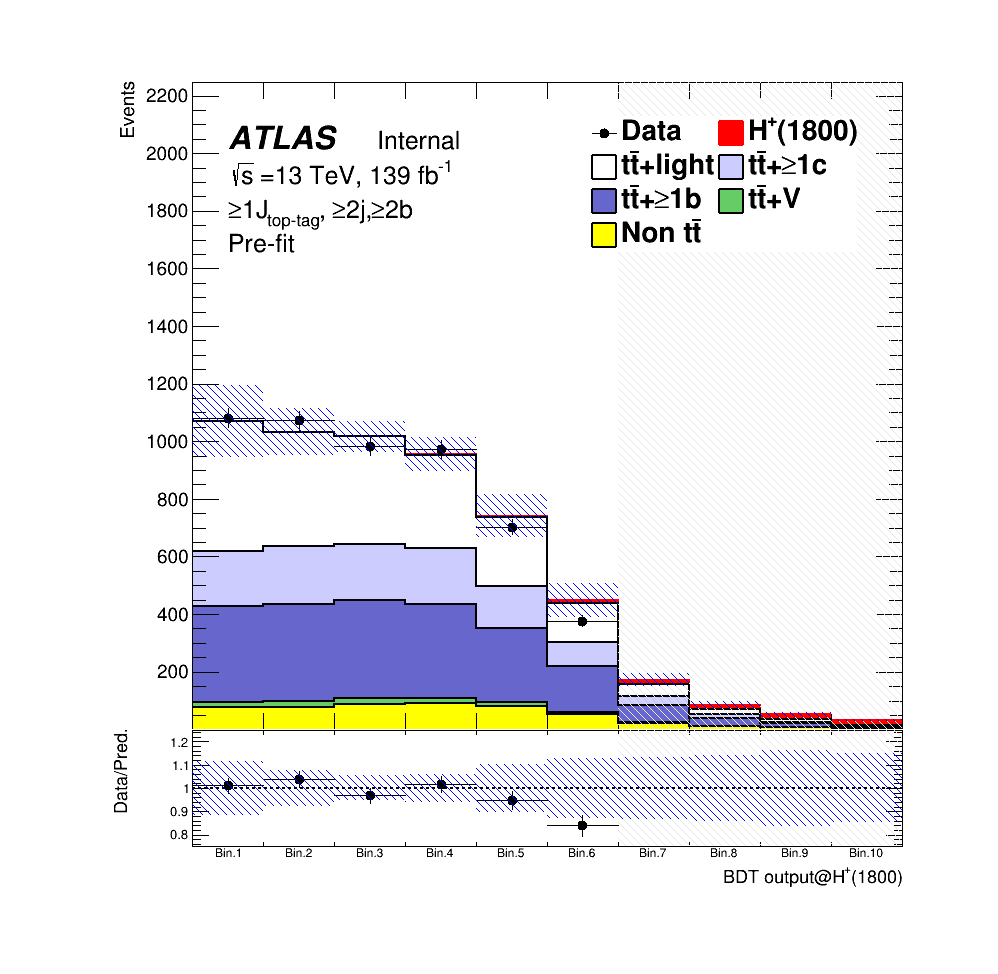
\includegraphics[width=0.50\textwidth]{images/BkgModeling/DATAOVERMC_Hp1800_Contained80_DL1r_70_bdt_Hp1800_beforeRW_geq1tgeq2jgeq2b_prefit.png}
        \label{fig:DataMCComparison_BDT_Hp1800_SR_beforeRW}
    }
    \subfloat[] {
        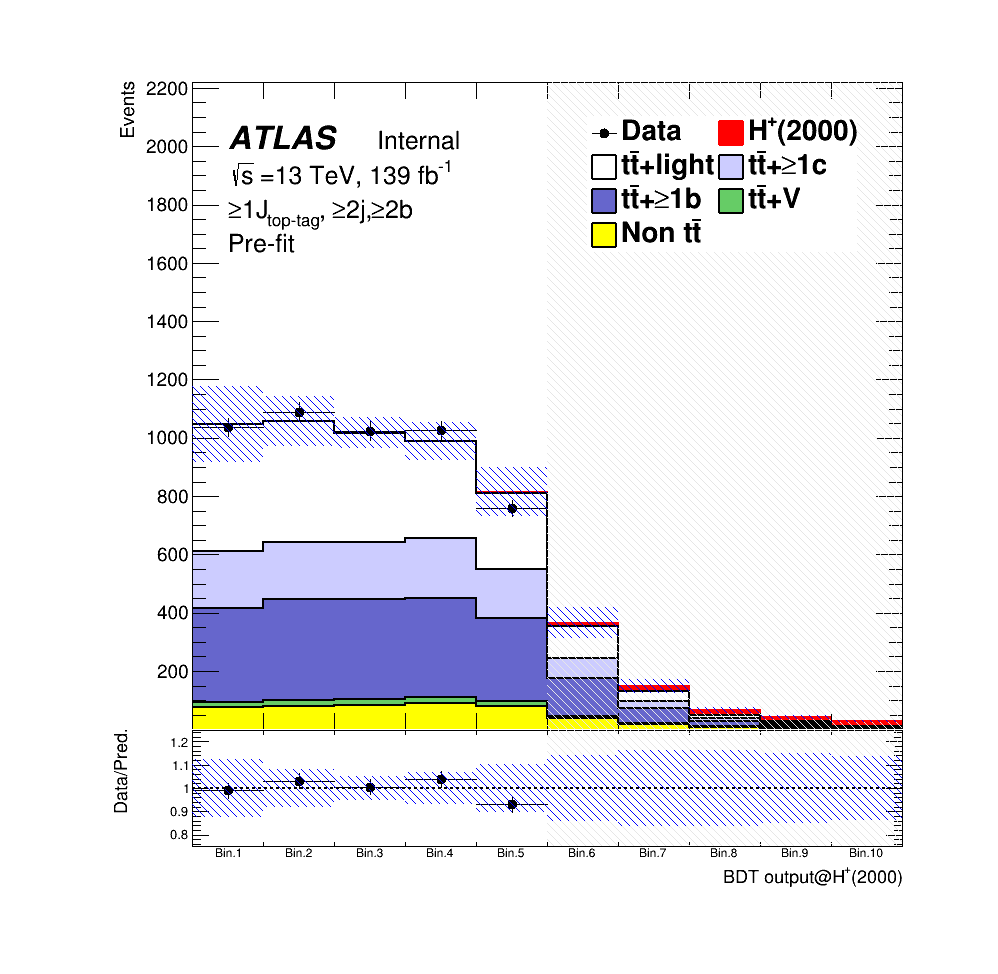
\includegraphics[width=0.50\textwidth]{images/BkgModeling/DATAOVERMC_Hp2000_Contained80_DL1r_70_bdt_Hp2000_beforeRW_geq1tgeq2jgeq2b_prefit.png}
        \label{fig:DataMCComparison_BDT_Hp2000_SR_beforeRW}
    }\par
    \subfloat[] {
        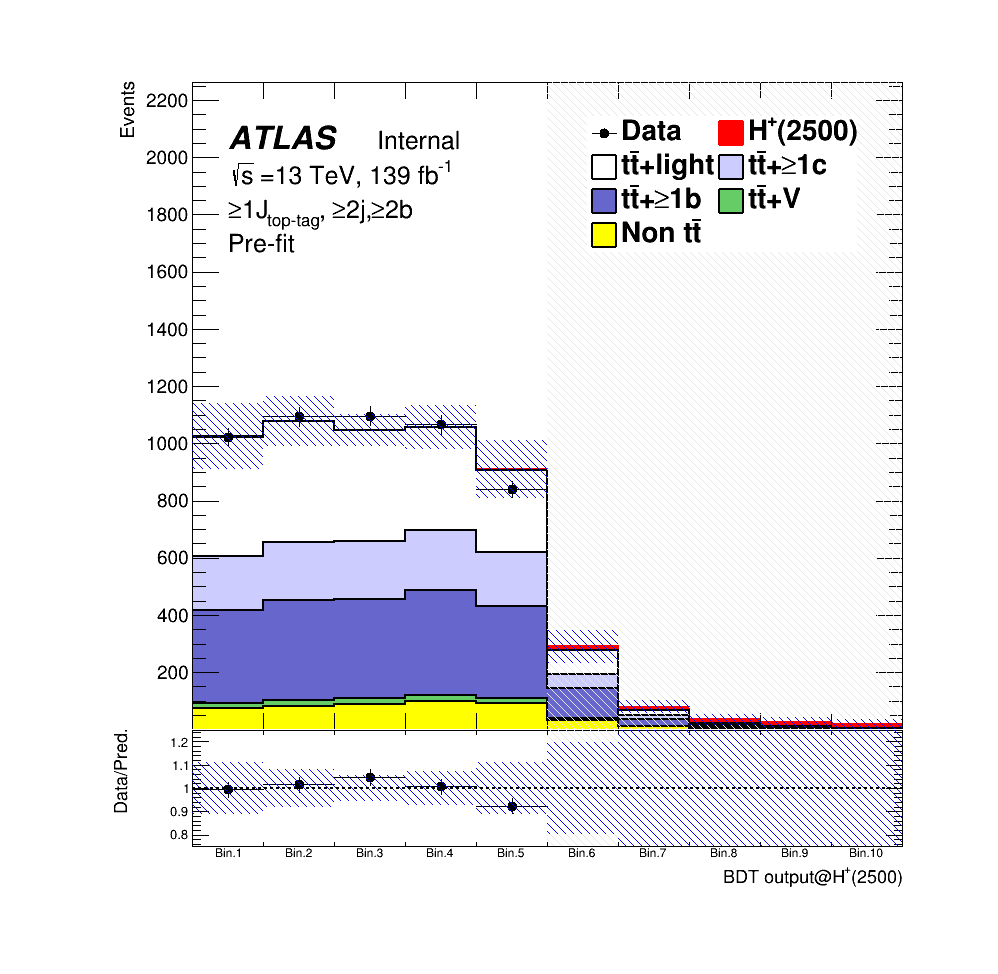
\includegraphics[width=0.50\textwidth]{images/BkgModeling/DATAOVERMC_Hp2500_Contained80_DL1r_70_bdt_Hp2500_beforeRW_geq1tgeq2jgeq2b_prefit.png}
        \label{fig:DataMCComparison_BDT_Hp2500_SR_beforeRW}
    }
    \subfloat[] {
        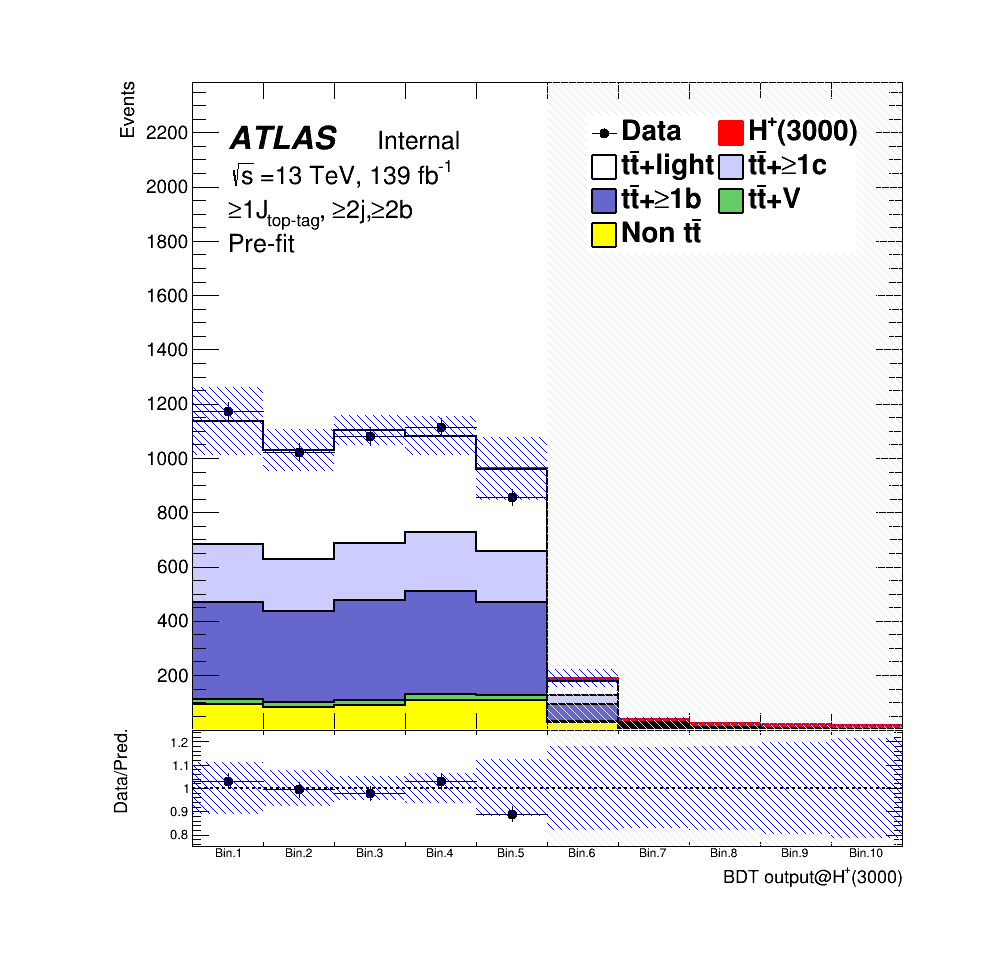
\includegraphics[width=0.50\textwidth]{images/BkgModeling/DATAOVERMC_Hp3000_Contained80_DL1r_70_bdt_Hp3000_beforeRW_geq1tgeq2jgeq2b_prefit.png}
        \label{fig:DataMCComparison_BDT_Hp3000_SR_beforeRW}
    }
    \caption{Pre-fit distribution of BDT output trained using from 1000 GeV (a) to 3000 GeV (h) $H^{+}$ samples in the SR.}
    \label{fig:DataMCComparison_BDT_beforeRW}
\end{figure}

\subsection{Reweighting technique}
\label{subsec:ReweightingTechnique}
Due to the mismodeling of the hard and soft jets, some extent of mis-modelling is expected in the $t\Bar{t}+\text{jets}$ samples generated by Powheg + Phytia. These mis-modelings appear, for example, in the number of jets, $p_\text{T}$ distribution of the leading top-tagged large-R jet (LeadingTop\_pt) and the invariant mass distribution of small-R jet triplet with maximum $p_{\text{T}}$ (Mjjj\_MaxPt) (these small-R jets are mainly QCD jets) as shown in Figure \ref{fig:DataMCComparison_In_LowBDTSocreRegion}.

\begin{figure}[H]
    \centering
    \subfloat[] {
        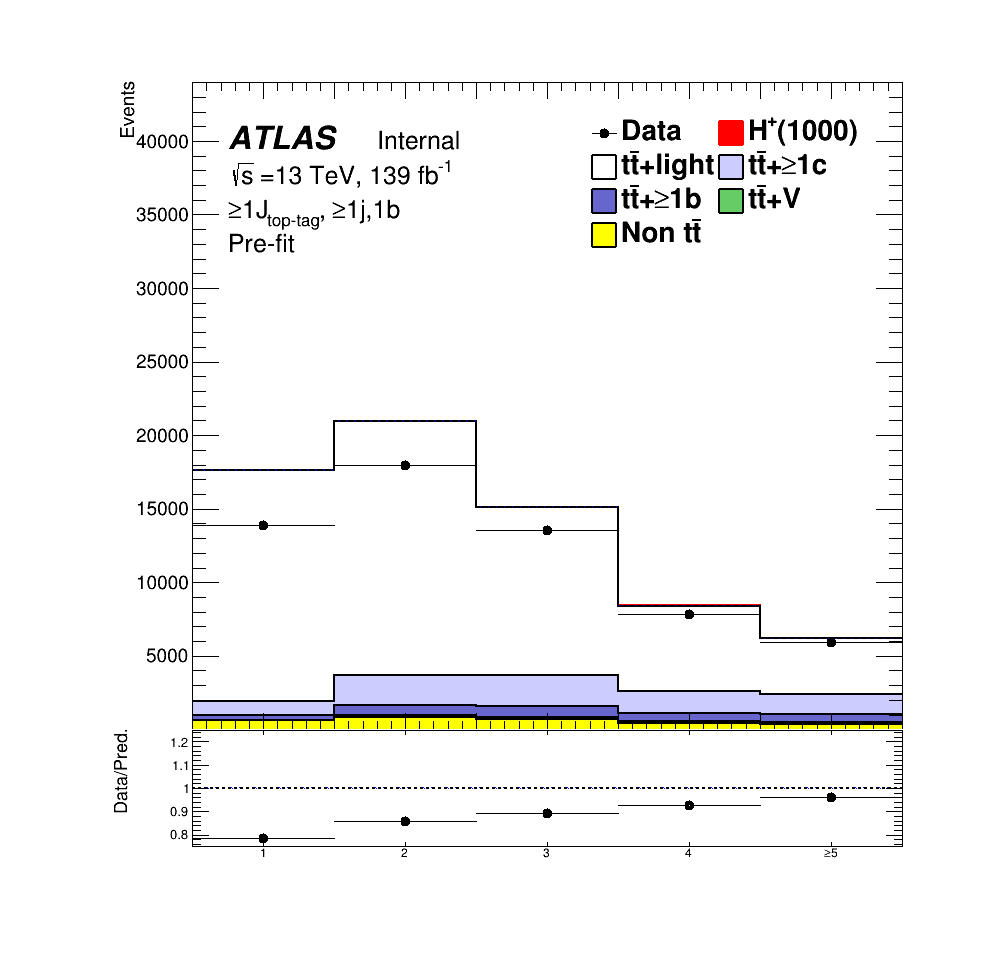
\includegraphics[width=0.50\textwidth]{images/BkgModeling/DATAOVERMC_Hp1000_Contained80_DL1r_70_nJets_beforeRW_geq1tgeq1j1b_prefit.png}
        \label{fig:nJets_CR}
    }\par
    \subfloat[] {
        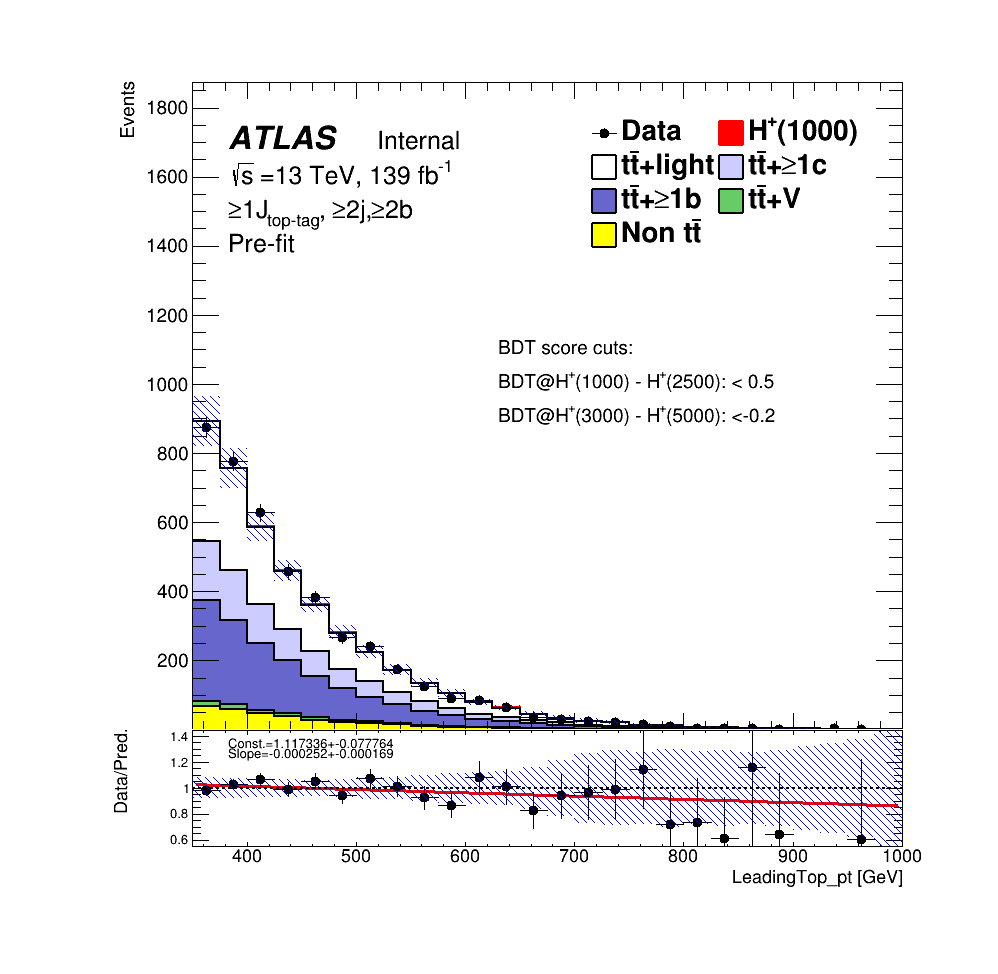
\includegraphics[width=0.50\textwidth]{images/BkgModeling/DATAOVERMC_Hp1000_Contained80_DL1r_70_LeadingTop_pt_LowBDTScore_beforeRW_geq1tgeq2jgeq2b_prefit.png}
        \label{fig:LeadingTop_pt_Modeling_LowBDTScoreEvents}
    }
    \subfloat[] {
        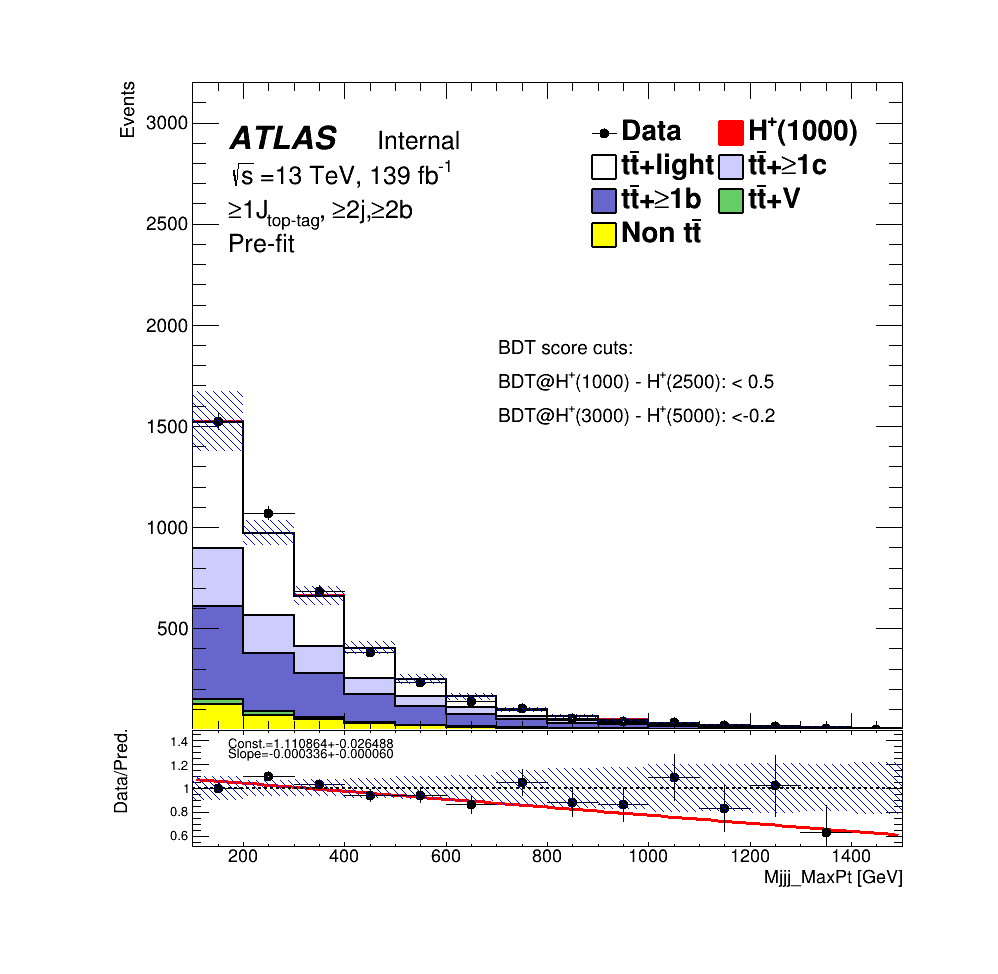
\includegraphics[width=0.50\textwidth]{images/BkgModeling/DATAOVERMC_Hp1000_Contained80_DL1r_70_Mjjj_MaxPt_LowBDTScore_beforeRW_geq1tgeq2jgeq2b_prefit.png}
        \label{fig:Mjjj_MaxPt_Modeling_LowBDTScoreEvents}
    }
    \caption{Number of jets in the CR (a), $p_{\text{T}}$ distribution of the leading top-tagged large-R jet in the SR (b) and invariant mass distribution of small-R jet triplet with maximum $p_{\text{T}}$ in the SR (c). These events in the SR are required to pass all BDT cuts shown in Table \ref{tab:ReqForRWControlRegion}. Each data/MC ratio plot has a slope.}
    \label{fig:DataMCComparison_In_LowBDTSocreRegion}
\end{figure}


To improve the prediction of $t\bar{t}+\text{jets}$, data-based corrections are applied to the MC prediction. The reweighing factors are derived by comparing the number of jets ($\text{N}_{\text{jets}}$) and $H_{\text{T}}^{\text{jets}}$ distributions between data and MC prediction. The reweighting factors for $\text{N}_{\text{jets}}$ are derived in the CR. Since the modelling is assumed to be due mainly to the additional radiation in the parton shower, which is independent on the flavour of associated jets, these reweighting factors are expected to improve the data/MC agreement in the SR as well, to the point that the remaining discrepancies would be well covered by the systematic model. The reweighting factors for $H_{\text{T}}^{\text{jets}}$ are derived in the SR and CR, individually, after reweighting with $\text{N}_{\text{jets}}$. When the reweighting factors are derived in the SR, events in the only low BDT score region are selected to avoid being reweighted signal events. These events are required to pass all the cuts shown in Table \ref{tab:ReqForRWControlRegion}. 

Firstly, the data/MC ratios $R$ are derived according to the following definition:
\begin{equation}
  R = \frac{\text{Data}-\text{MC}^{\text{non-}t\bar{t}+\text{jets}}}{f \cdot \text{MC}^{t\bar{t}+\text{jets}}}
\end{equation}

$t\bar{t}+\text{jets}$ includes the $t\bar{t}+\text{light}$, $t\bar{t}+\geq1c$ and $t\bar{t}+\geq1b$. The number of $t\bar{t}+\text{jets}$ MC events is scaled by $f$ to the number of data subtracted non $t\bar{t}+\text{jets}$ MC events. Figure \ref{fig:RWFactors_Njets_CR} shows the number of jets and data/MC ratio, $R$, distributions. The first reweighting is performed using the $R$ in each $\text{N}_{\text{jets}}$ bin, which is applied to $t\bar{t}+\text{light}$, $t\bar{t}+\geq1c$ and $t\bar{t}+\geq1b$. Figure \ref{fig:RWFactors_HTjets} shows the $H_{\text{T}}^{\text{jets}}$ and $R$ distributions in each SR and CR after reweighting with $\text{N}_{\text{jets}}$. When the $R$ is derived in the SR, events in the only low BDT score region are selected to avoid being reweighted signal events according to Table \ref{tab:ReqForRWControlRegion}. These obtained $R$ distributions are fitted with a quadratic function ($f(H_{\text{T}}^{\text{jets}}) = a + b \cdot H_{\text{T}}^{\text{jets}} + c \cdot (H_{\text{T}}^{\text{jets}})^{2}$, where $a$, $b$, and $c$ are free parameters determined in the fit), and the function is used for reweighting. The function is applied to $t\bar{t}+\text{light}$, $t\bar{t}+\geq1c$ and $t\bar{t}+\geq1b$ as well as $\text{N}_{\text{jets}}$ reweighting. The obtained reweighting functions are also shown in Figure \ref{fig:RWFactors_HTjets}. Table \ref{tab:ParameterOfReweightingFunction} includes the fitted values for all the parameters. The statistical errors of fitted parameters are included as systematic uncertainties in the final fitting. The reweighting factors in $H_{\text{T}}^{\text{jets}}>2072$ GeV region are used the value at $H_{\text{T}}^{\text{jets}}=2072$ GeV because the weight value of $-1\sigma$ become negative at the point.

\begin{table}[H]
  \centering
  \begin{tabular*}{70mm}{@{\extracolsep{\fill}}cc}
    \hline\hline
    Mass point [GeV] & BDT score cut\\
    \hline
    1000             & $< 0.5$\\
    1200             & $< 0.5$\\
    1400             & $< 0.5$\\
    1600             & $< 0.5$\\
    1800             & $< 0.5$\\
    2000             & $< 0.5$\\
    2500             & $< 0.5$\\
    3000             & $<-0.2$\\
    4000             & $<-0.2$\\
    5000             & $<-0.2$\\
    \hline\hline
  \end{tabular*}
  \caption{Requirements on the events used for reweighting factor calculation in the SR. These cuts are defined so that events are derived from the regions with S/N $<$ 0.05 for any mass points.}
  \label{tab:ReqForRWControlRegion}
\end{table}

\begin{figure}[H]
    \centering
    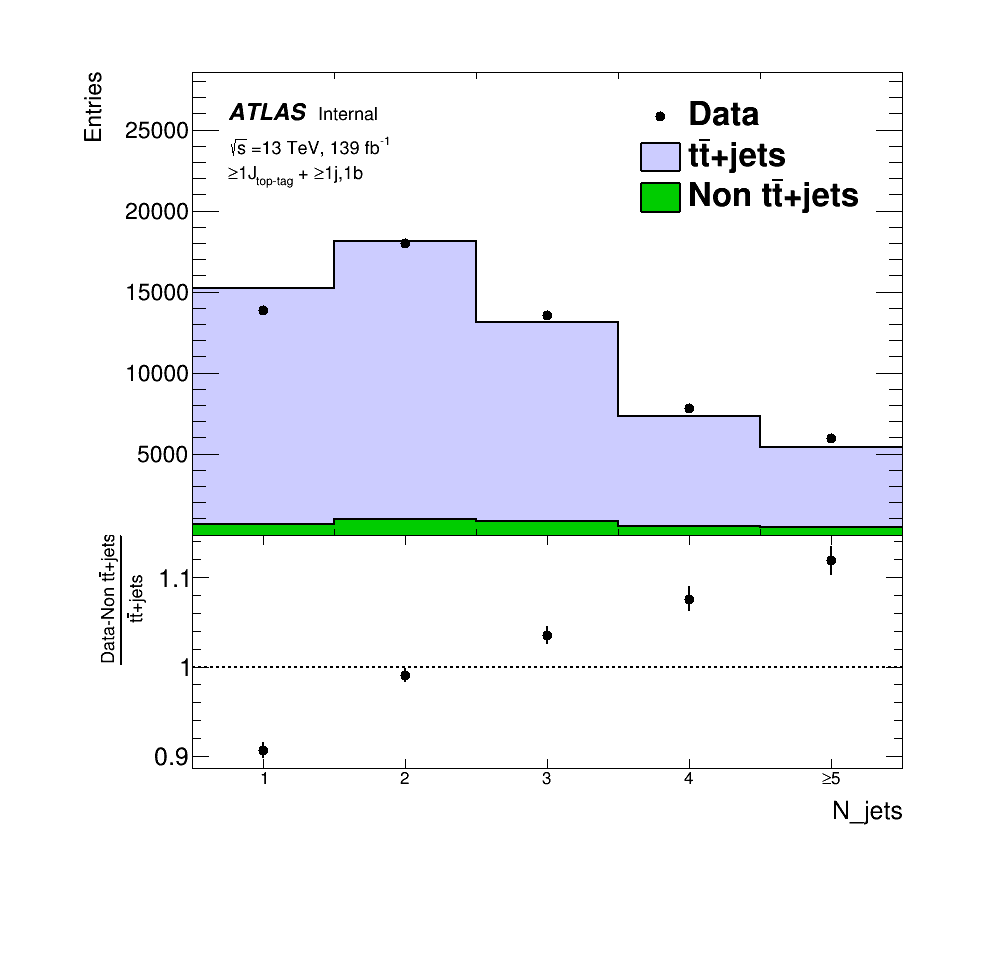
\includegraphics[width=0.50\textwidth]{images/BkgModeling/RWFactors_Njets.png}
    \caption{Number of jets (top canvas) and data/MC ratio, $R$, (bottom canvas) distributions. The first reweighting is performed using the $R$ in each $\text{N}_{\text{jets}}$ bin, , which is applied to $t\bar{t}+\text{light}$, $t\bar{t}+\geq1c$ and $t\bar{t}+\geq1b$.}
    \label{fig:RWFactors_Njets_CR}
\end{figure}

\begin{figure}[H]
  \subfloat[] {
    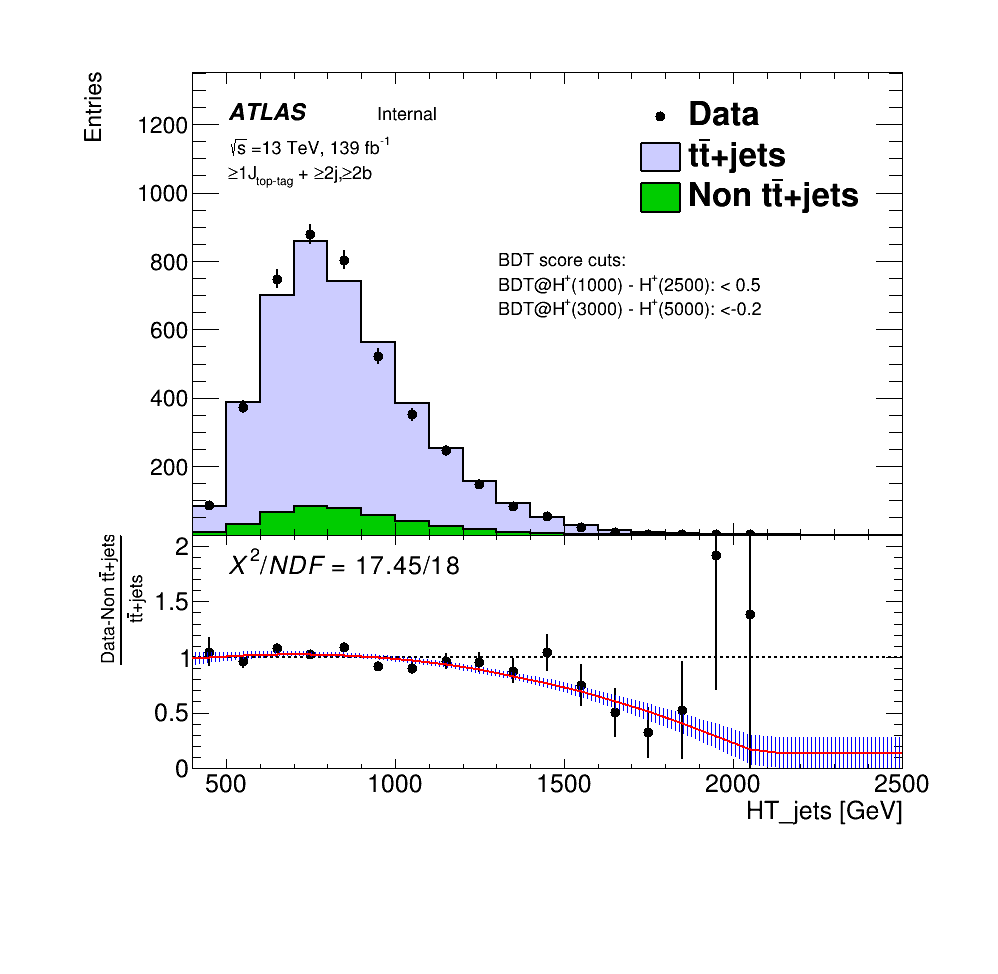
\includegraphics[width=0.50\textwidth]{images/BkgModeling/RWFactors_HTjets_SR.png}
    \label{fig:HTjets_LowBDTScoreRegion}
  }
  \subfloat[] {
    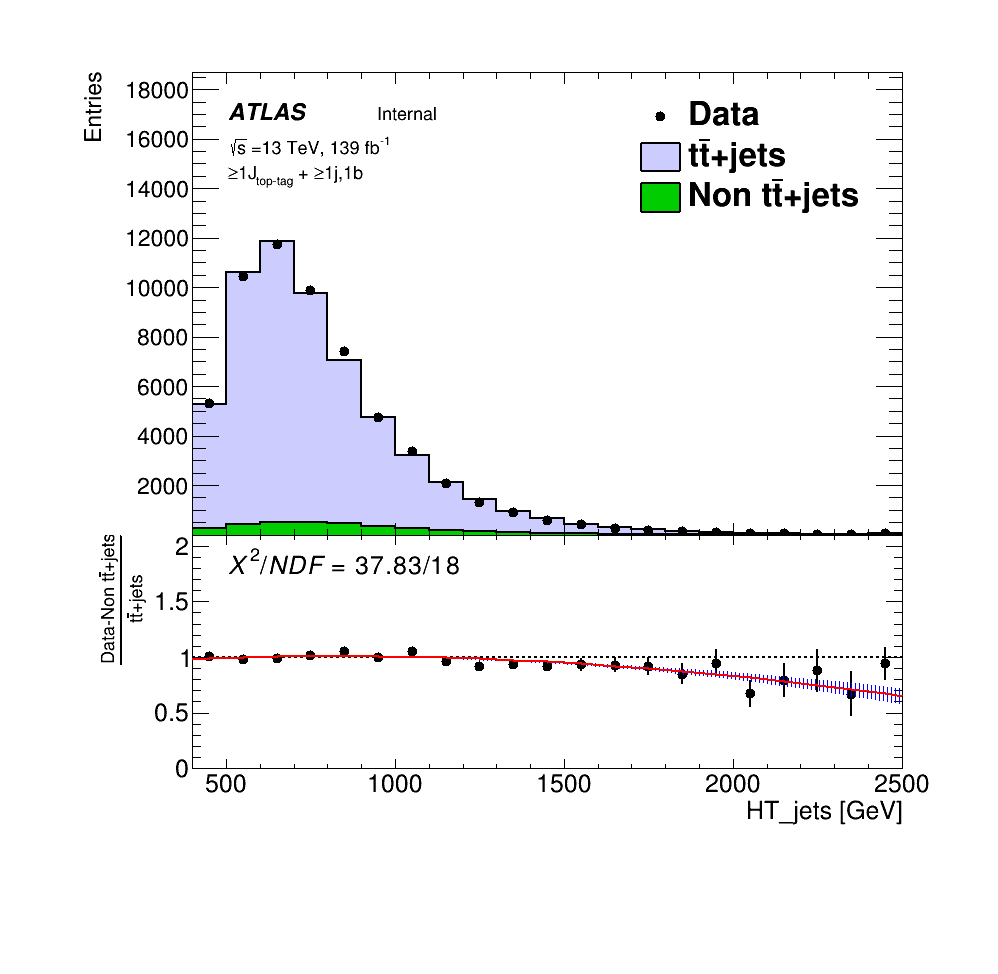
\includegraphics[width=0.50\textwidth]{images/BkgModeling/RWFactors_HTjets_CR.png}
    \label{fig:HTjets_WeightFactor}
  }
  \caption{$H_{\text{T}}^{\text{jets}}$ and data/MC ratio, $R$, distributions in the SR (a) and CR (b). The events in the SR are selected by BDT score. The red functions in the bottom canvases are the reweighting functions obtained by fitting to $R$ distribution with a quadratic function. The blue bands are the statistical uncertainty (${\pm}1{\sigma}$) of the red function. They are included as systematic uncertainties in the final fitting. For events with $H_{\text{T}}^{\text{jets}}>2072$ GeV in the SR, the same weight and its error as region $H_{\text{T}}^{\text{jets}}=2072$ GeV is given. }
  \label{fig:RWFactors_HTjets}
\end{figure}


\begin{table}[H]
  \centering
  \begin{tabular*}{120mm}{c|c|c}
    \hline\hline
    Parameter & Value (SR)                      & Value (CR)\\
    \hline
    $a$       & $( 7.95{\pm}1.45)\times10^{-1}$ & $( 9.20{\pm}0.32)\times10^{-1}$\\
    \hline
    $b$       & $( 6.70{\pm}2.82)\times10^{-4}$ & $( 2.14{\pm}0.67)\times10^{-4}$\\
    \hline
    $c$       & $(-4.75{\pm}1.29)\times10^{-7}$ & $(-1.29{\pm}0.32)\times10^{-7}$\\
    \hline\hline
  \end{tabular*}
  \caption{Summary of parameters obtained by fitting of a quadratic function in the SR and CR ($f(H_{\text{T}}^{\text{jets}}) = a + b \cdot H_{\text{T}}^{\text{jets}} + c \cdot (H_{\text{T}}^{\text{jets}})^{2}$). The error of each parameter is from statistical uncertainty.}
  \label{tab:ParameterOfReweightingFunction}
\end{table}


Figure \ref{fig:BDT_Hp1000_AfterRW} to Figure \ref{fig:BDT_Hp3000_AfterRW} show BDT output distributions applied to reweighting in the SR. The data/MC agreement in the high BDT score regions is improved.

\begin{figure}[H]
    \subfloat[] {
        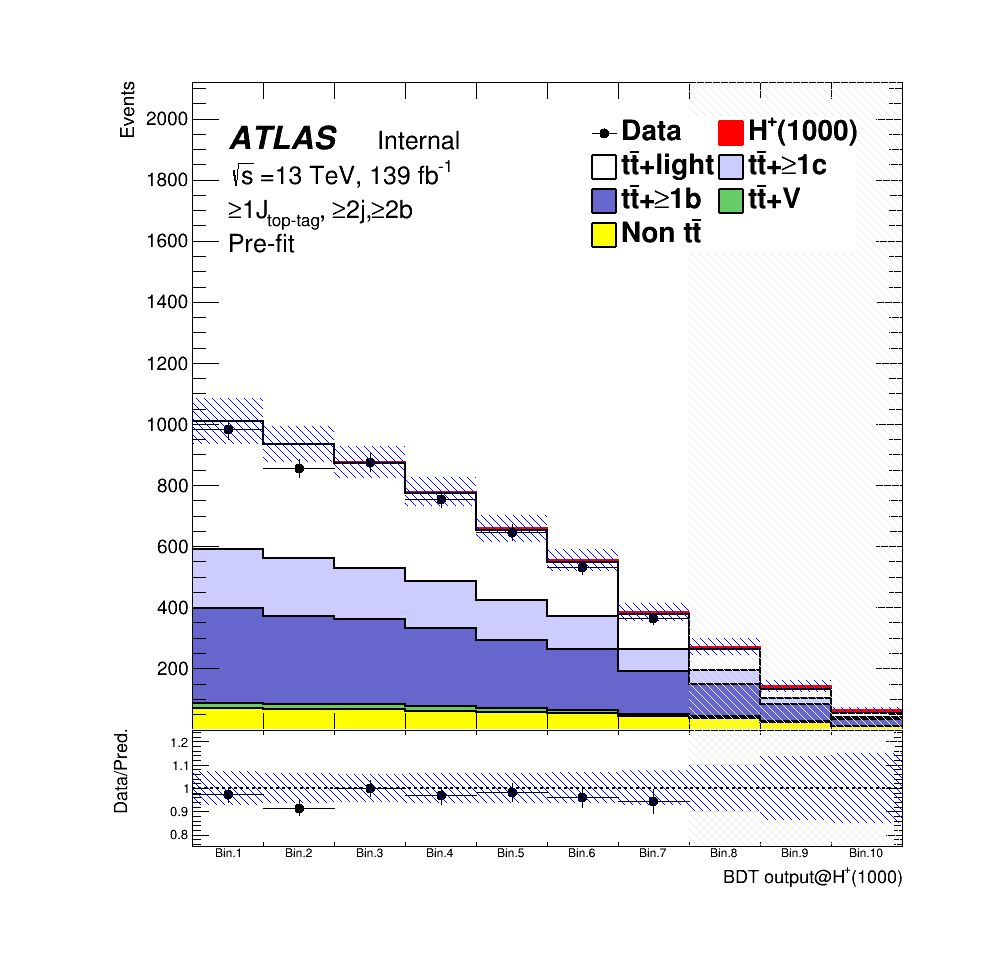
\includegraphics[width=0.50\textwidth]{images/BkgModeling/DATAOVERMC_Hp1000_Contained80_DL1r_70_bdt_Hp1000_geq1tgeq2jgeq2b_prefit.png}
        \label{fig:BDT_Hp1000_AfterRW}
    }
    \subfloat[] {
        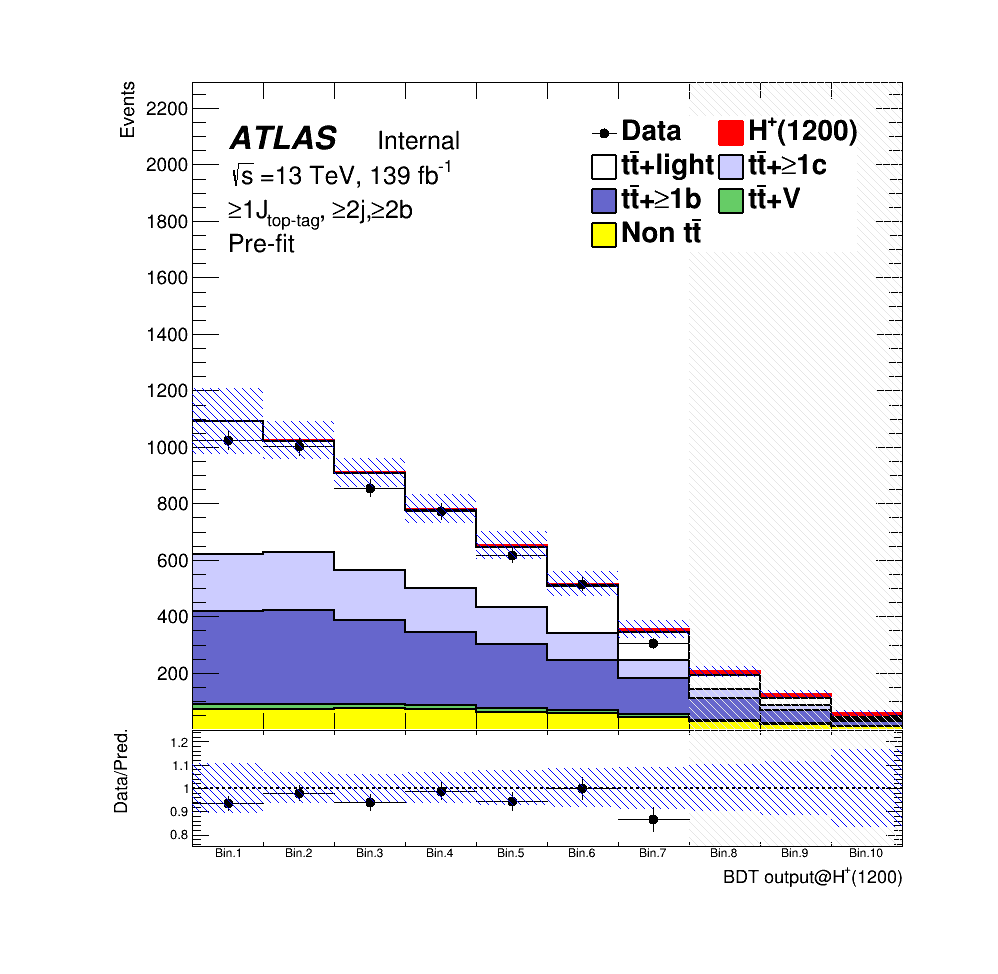
\includegraphics[width=0.50\textwidth]{images/BkgModeling/DATAOVERMC_Hp1200_Contained80_DL1r_70_bdt_Hp1200_geq1tgeq2jgeq2b_prefit.png}
        \label{fig:BDT_Hp1200_AfterRW}
    }\par
    \subfloat[] {
        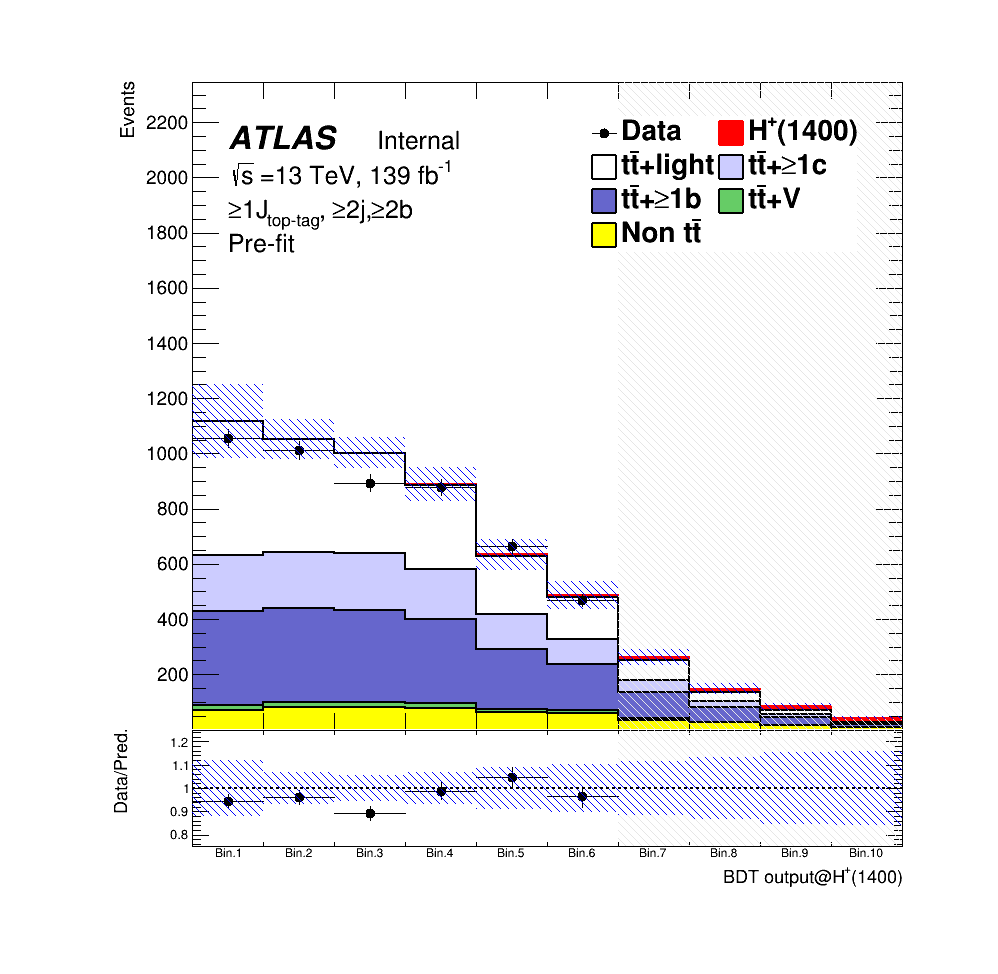
\includegraphics[width=0.50\textwidth]{images/BkgModeling/DATAOVERMC_Hp1400_Contained80_DL1r_70_bdt_Hp1400_geq1tgeq2jgeq2b_prefit.png}
        \label{fig:BDT_Hp1400_AfterRW}
    }
    \subfloat[] {
        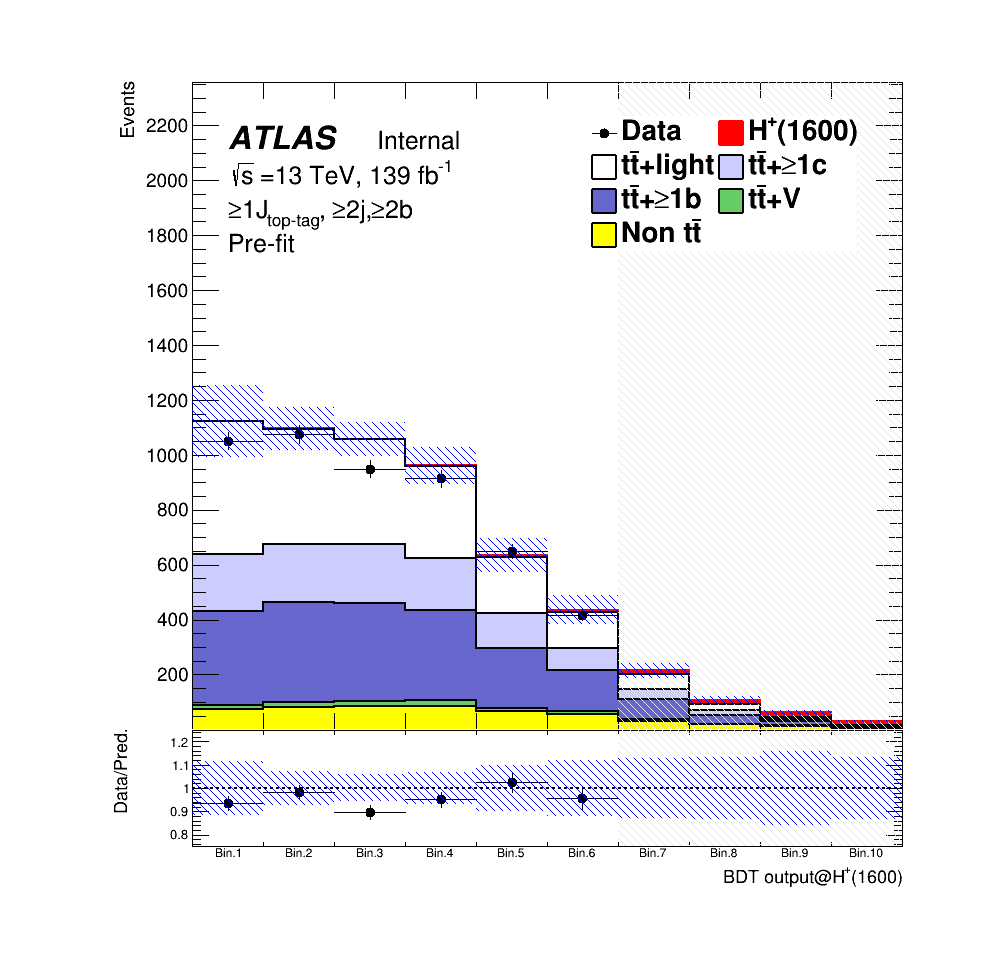
\includegraphics[width=0.50\textwidth]{images/BkgModeling/DATAOVERMC_Hp1600_Contained80_DL1r_70_bdt_Hp1600_geq1tgeq2jgeq2b_prefit.png}
        \label{fig:BDT_Hp1600_AfterRW}
    }
\end{figure}
\begin{figure}[H]
    %\addtocounter{figure}{-1}
    \subfloat[] {
        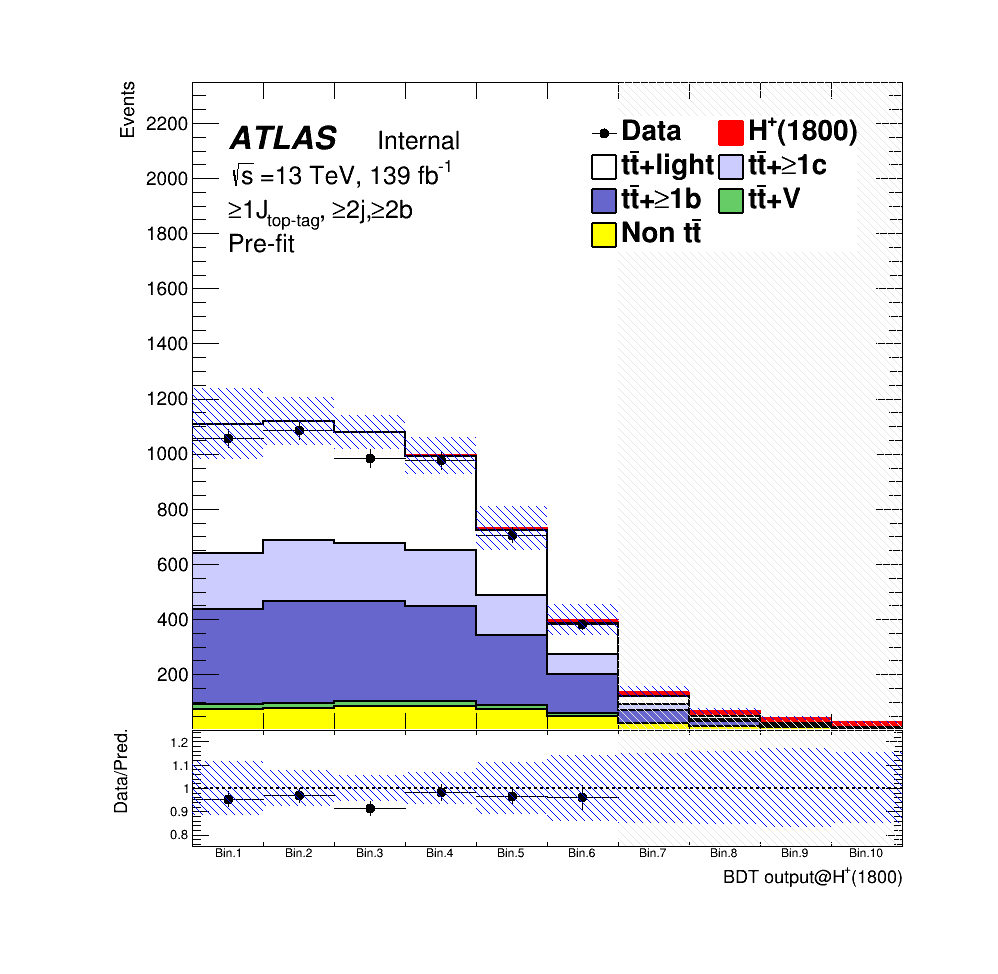
\includegraphics[width=0.50\textwidth]{images/BkgModeling/DATAOVERMC_Hp1800_Contained80_DL1r_70_bdt_Hp1800_geq1tgeq2jgeq2b_prefit.png}
        \label{fig:BDT_Hp1800_AfterRW}
    }
    \subfloat[] {
        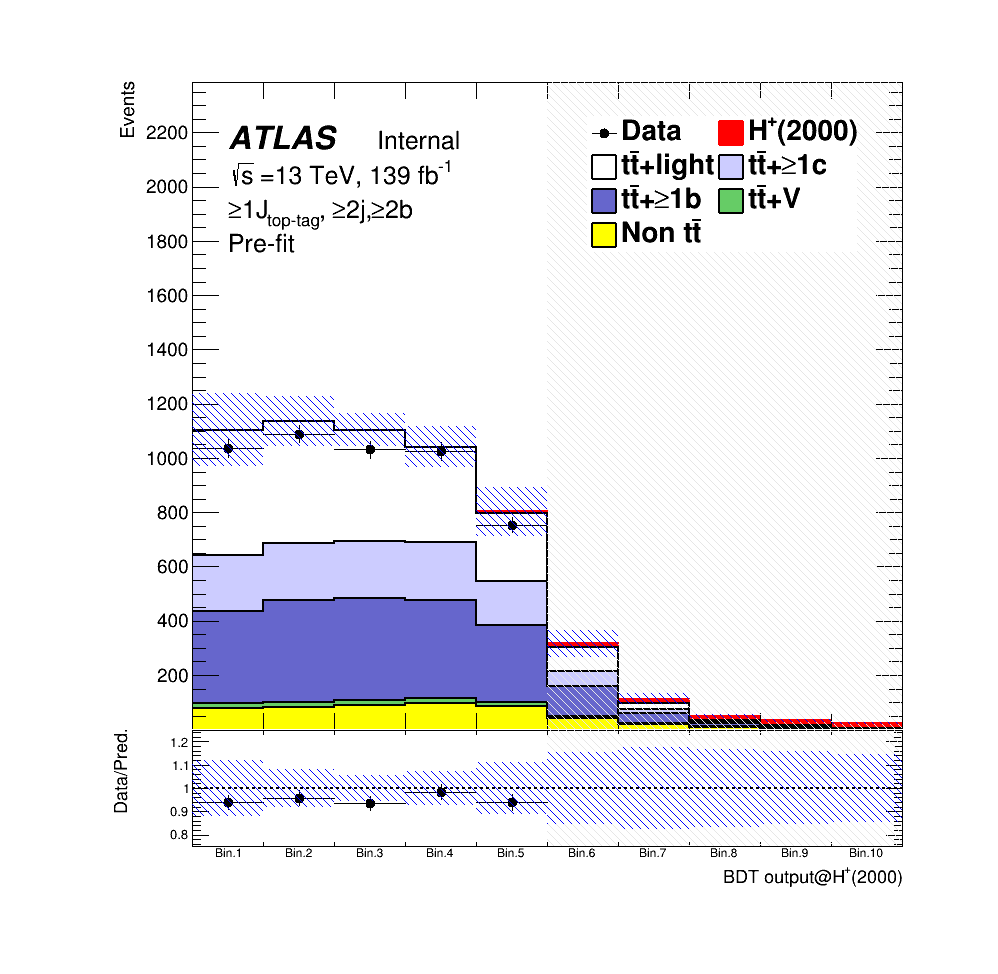
\includegraphics[width=0.50\textwidth]{images/BkgModeling/DATAOVERMC_Hp2000_Contained80_DL1r_70_bdt_Hp2000_geq1tgeq2jgeq2b_prefit.png}
        \label{fig:BDT_Hp2000_AfterRW}
    }\par
    \subfloat[] {
        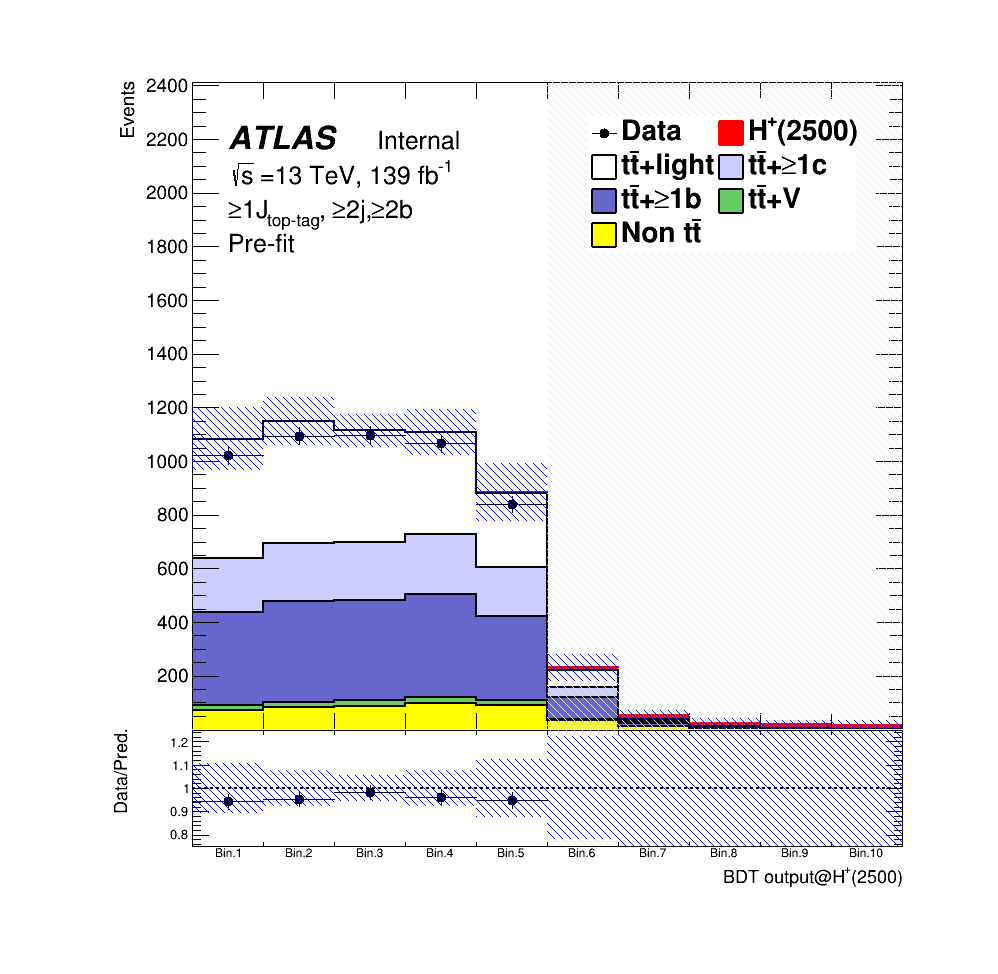
\includegraphics[width=0.50\textwidth]{images/BkgModeling/DATAOVERMC_Hp2500_Contained80_DL1r_70_bdt_Hp2500_geq1tgeq2jgeq2b_prefit.png}
        \label{fig:BDT_Hp2500_AfterRW}
    }
    \subfloat[] {
        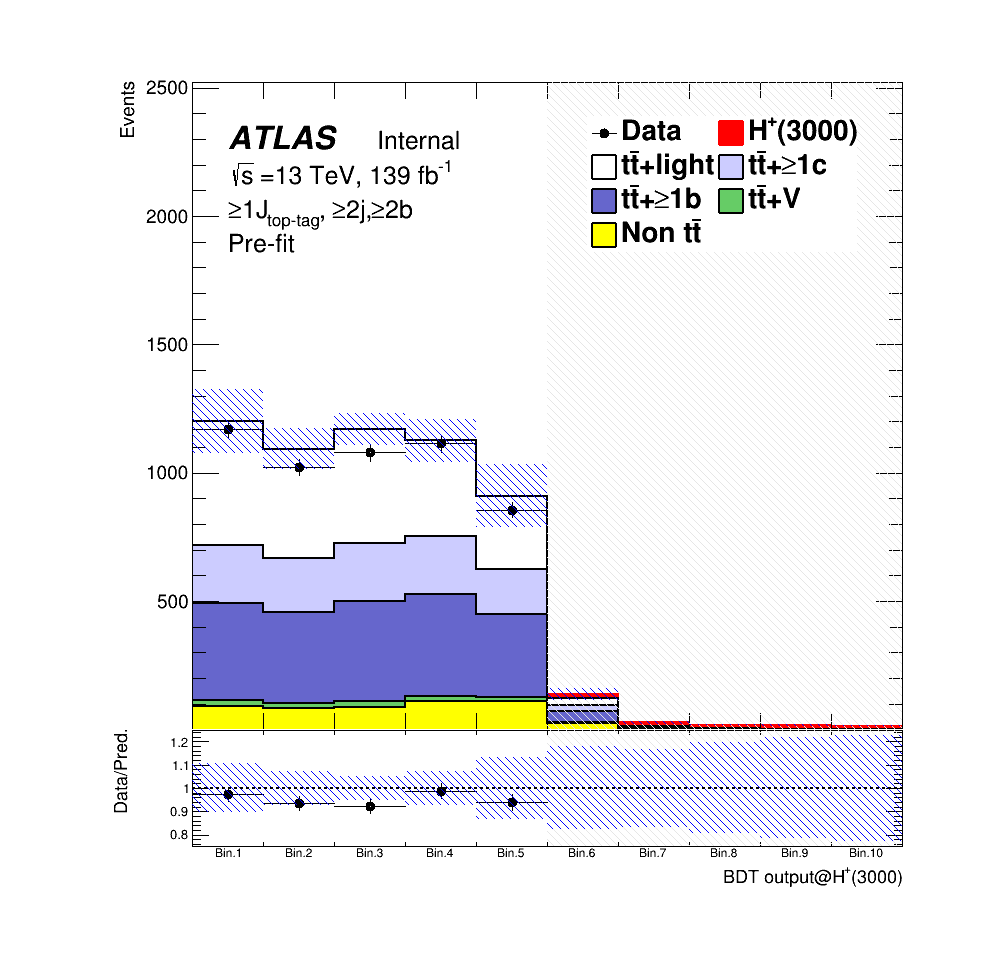
\includegraphics[width=0.50\textwidth]{images/BkgModeling/DATAOVERMC_Hp3000_Contained80_DL1r_70_bdt_Hp3000_geq1tgeq2jgeq2b_prefit.png}
        \label{fig:BDT_Hp3000_AfterRW}
    }
    \caption{Pre-fit distributions of BDT output trained using from 1000 (a) to 3000 (h) GeV $H^{+}$ in the SR after reweighting.}
    \label{fig:BDT_AfterRW}
\end{figure}